\باب{برقی اور میکانی توانائی کا باہمی تبادلہ}
%proof read the entire chapter
برقی رو یا مقناطیسی بہاو کی مدد سے برقی توانائی کو میکانی توانائی یا میکانی توانائی کو برقی توانائی میں مختلف مشین تبدیل کرتے ہیں۔ پیمائشی آلات، لاؤڈ سپیکر، مائکروفون، وغیرہ  نہایت کم طاقت کا تبادلہ کرتے ہیں جبکہ  \اصطلاح{ریلے}\فرہنگ{ریلے}\حاشیہب{relay}\فرہنگ{relay}، برقی مقناطیس، وغیرہ،  قوت پیدا کرتے ہیں۔ کئی مشین، جن میں برقی موٹر اور جنریٹر شامل ہیں،   ایک قسم کی توانائی کو  دوسری قسم کی توانائی میں مسلسل تبدیل کرتے ہیں۔

اس باب میں مقناطیسی بہاو کی مدد سے توانائی کے تبادلہ پر غور کیا جائے گا۔برقی رو کی مدد سے بھی توانائی کا تبادلہ سمجھا جا سکتا ہے جس کا تذکرہ اس کتاب میں نہیں کیا جائے گا۔

اس باب میں ہم وہ اہم تراکیب سیکھیں گے جو انجنیئری مسائل حل کرنے میں مددگار ثابت ہوں گے۔

\حصہ{مقناطیسی نظام میں قوت  اور  قوت مروڑ}
برقی میدان \عددی{\kvec{E}} میں برقی بار \عددیء{q}  پر درج ذیل قوت اثر انداز ہو گی۔
\begin{align}\label{مساوات_تبادلہ_برقی_میدان_قوت}
\kvec{F}=q \kvec{E}
\end{align}
مثبت برقی بار پر قوت  برقی شدت \سمتیہ{E} کے رخ ہو گی جبکہ منفی  بار پر قوت \سمتیہ{E} کے مخالف رخ ہو گی۔

مقناطیسی میدان میں متحرک بار \عددی{q}، جس کی \اصطلاح{سمتی رفتار}\فرہنگ{سمتی رفتار}\حاشیہب{velocity} \سمتیہ{v} ہو، پر  درج ذیل قوت اثر انداز ہو گی۔
\begin{align}\label{مساوات_برقی_میکانی_تبادلہ_مقناطیسی}
\kvec{F}=q \left(\kvec{v} \times \kvec{B} \right)
\end{align}
مثبت برقی بار پر  قوت کا رخ  \اصطلاح{دائیں ہاتھ کا قانون}\حاشیہب{right hand rule} دیگا (شکل \حوالہ{شکل_تبادلہ_توانائی_دائیں_ہاتھ_قانون})۔دائیں ہاتھ کے انگوٹھے  کو باقی انگلیوں کے ساتھ برقرار قائمہ رکھ کر اس ہاتھ کی چار انگلیوں کو \عددی{\kvec{v}} کے رخ سے شروع کر کے، چھوٹے زاویہ پر گھما کر،  \عددی{\kvec{B}} کے رخ  موڑنے سے انگوٹھا \عددی{\kvec{F}} کا رخ دیگا۔ منفی بار پر قوت  مخالف رخ ہو گی۔

\begin{figure}
\centering
\begin{tikzpicture}
    \node[anchor=south west,inner sep=0] (image) at (0,0) {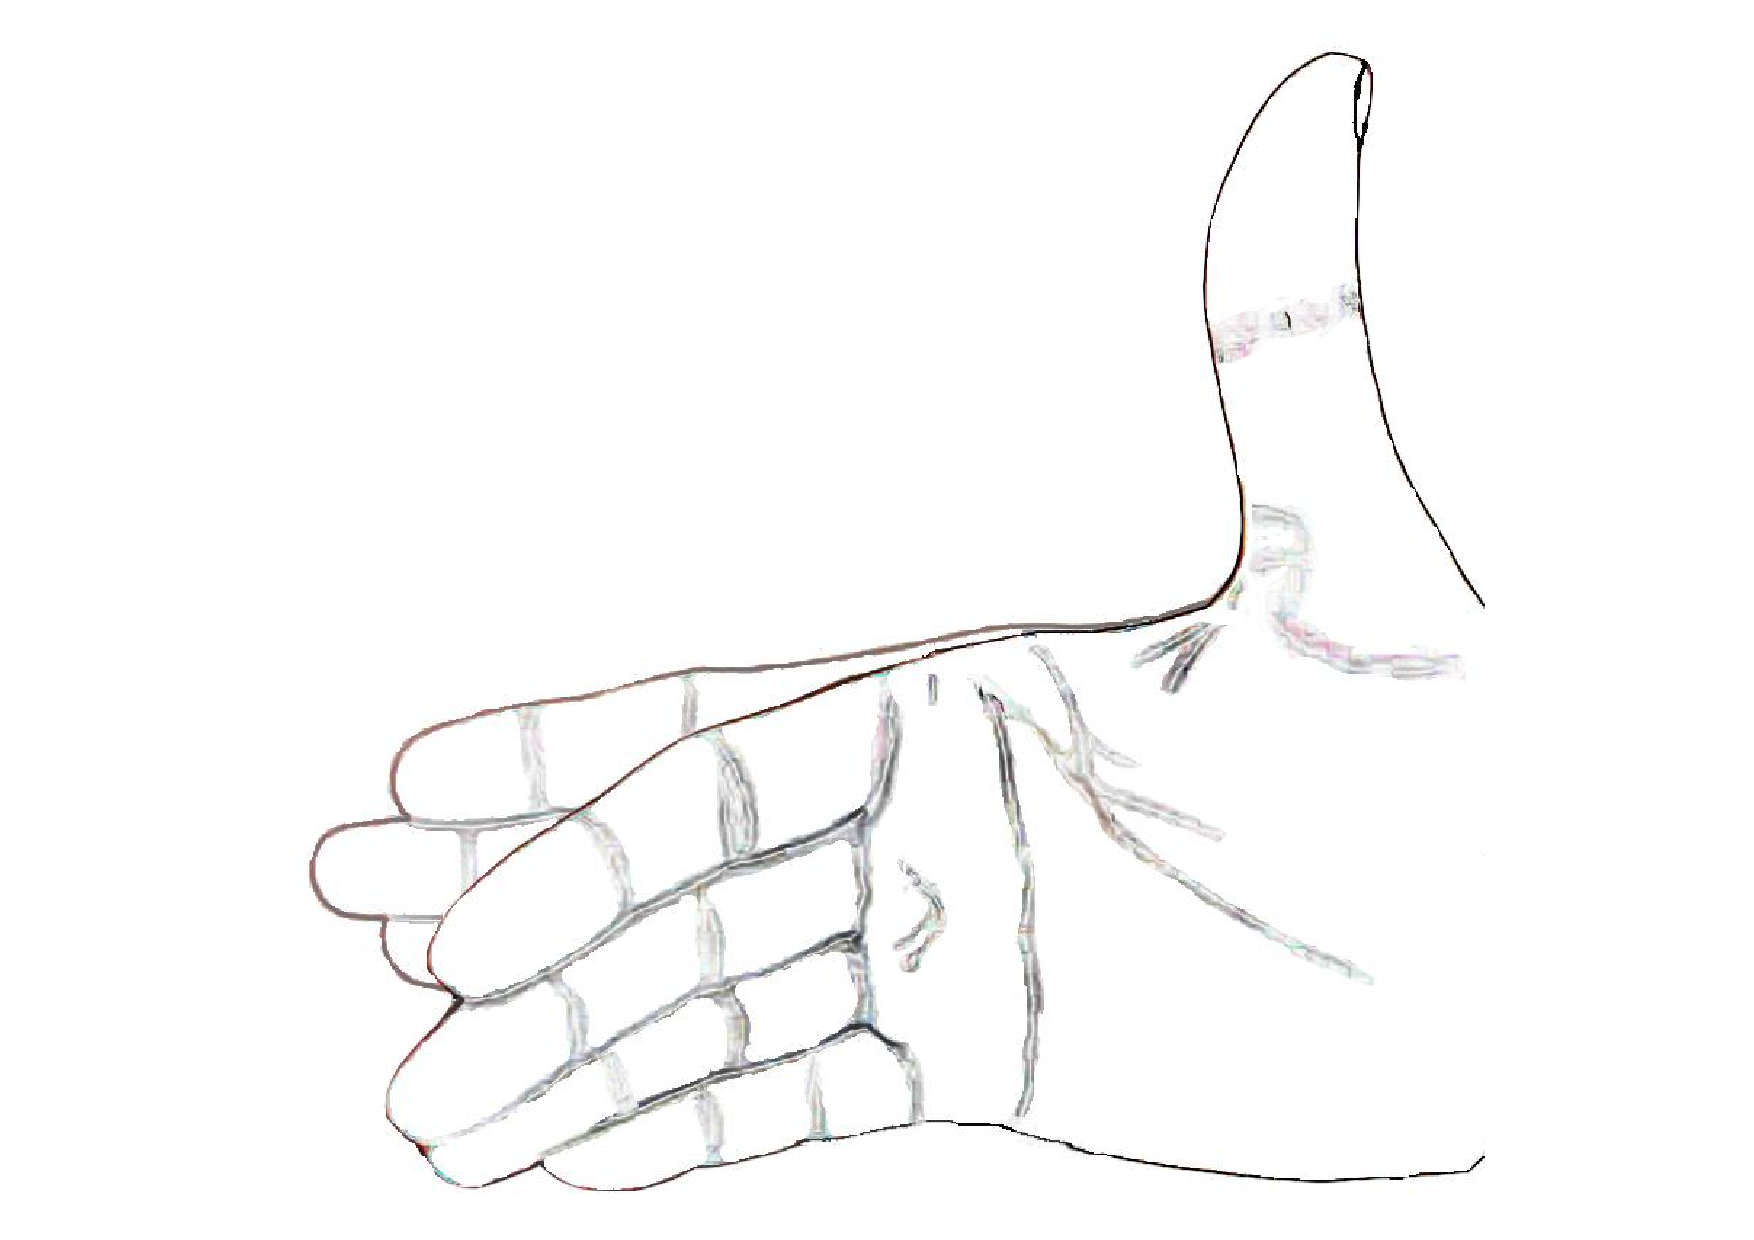
\includegraphics[height=3.5cm]{figEnergyConversionRightHandForceRule}};
    \begin{scope}[x={(image.south east)},y={(image.north west)}]
 %\draw[red,step=0.1] (0,0) grid (1,1);
\draw[-latex](0.16,0.3)--++(-0.2,0)node[left]{$\kvec{v}$};
\draw[-latex](0.2,0.1)--++(-0.1,-0.1)node[left]{$\kvec{B}$};
\draw[-latex](0.65,0.7)--++(0,0.2)node[left]{$\kvec{F}$};
    \end{scope}
\end{tikzpicture}
%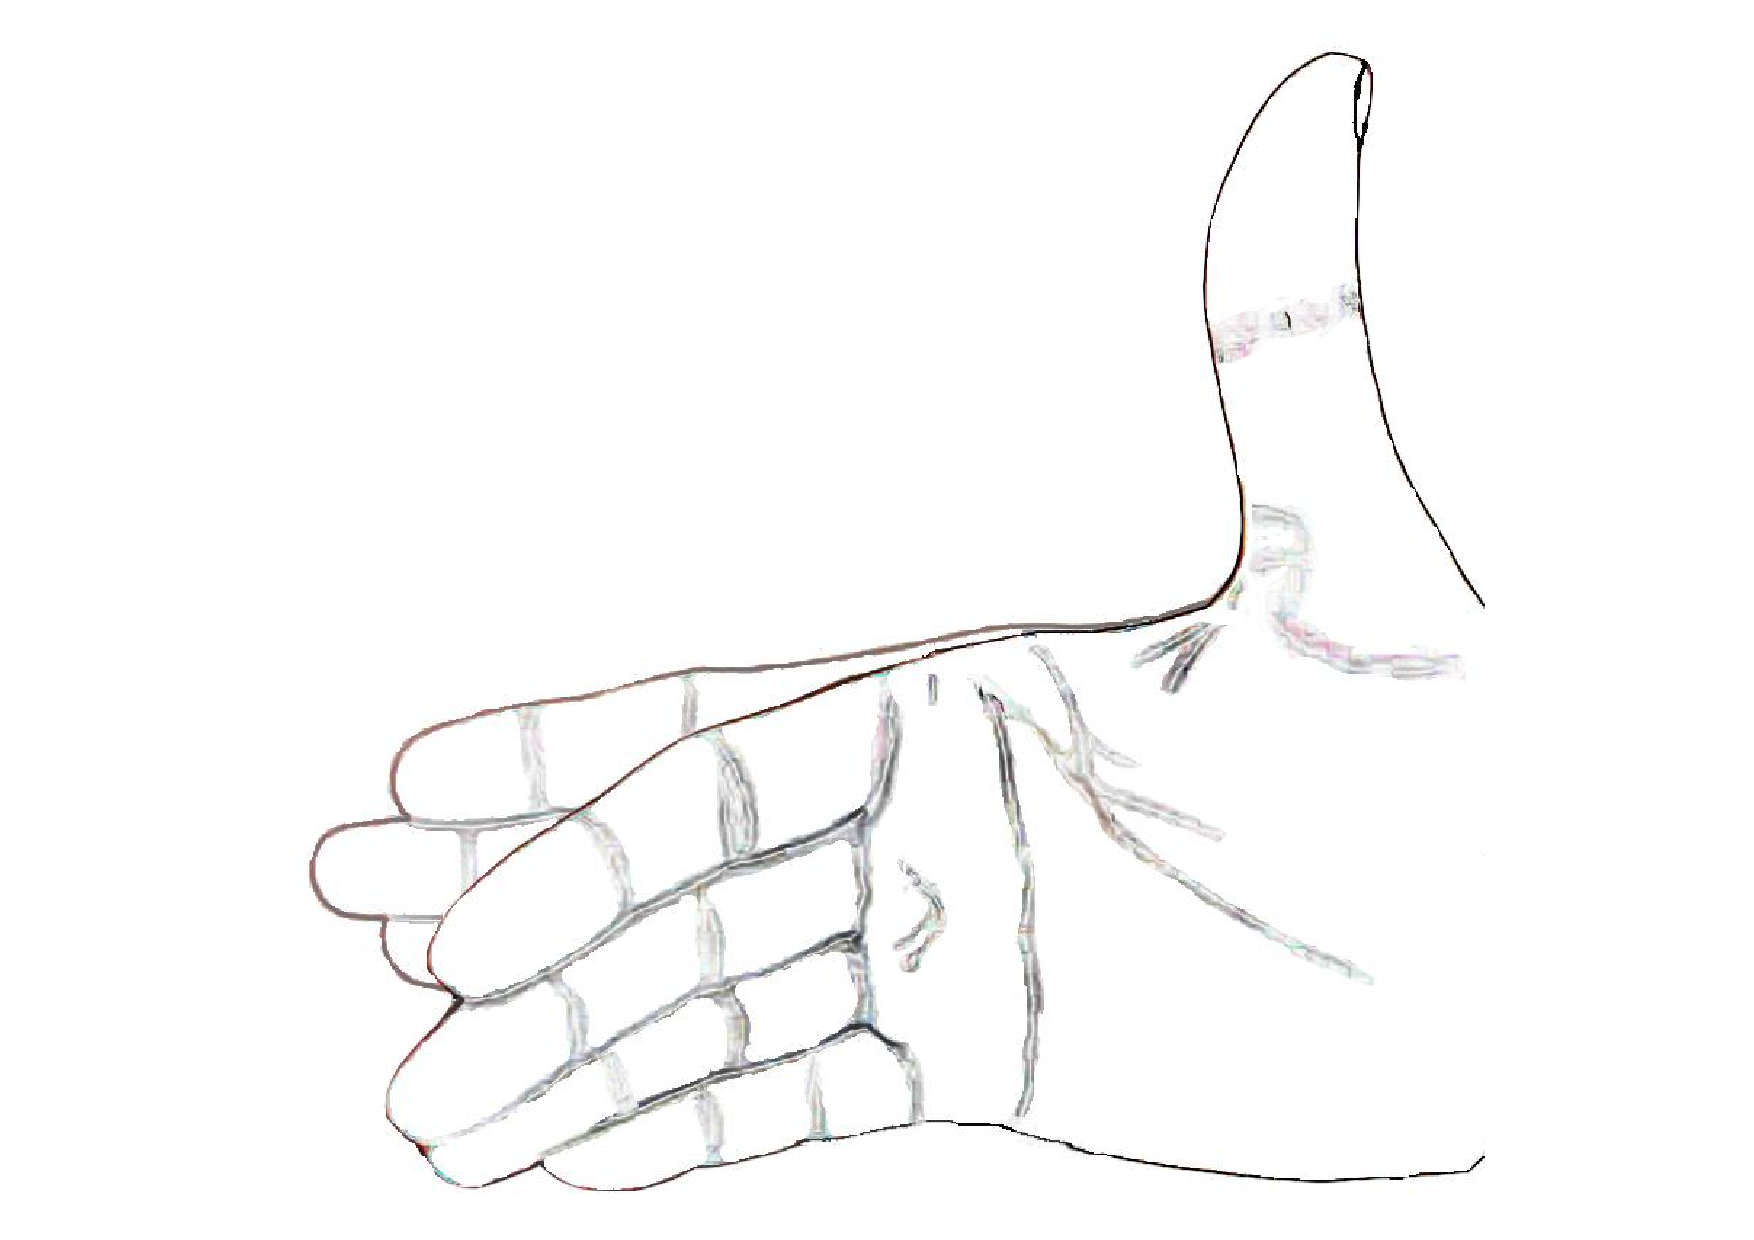
\includegraphics[height=3.5cm]{figEnergyConversionRightHandForceRule}
\caption{
دائیں ہاتھ کی چار انگلیوں کو \عددی{\kvec{v}} سے \عددی{\kvec{B}} کی طرف کم زاویہ پر موڑیں۔ اس ہاتھ کا انگوٹھا قوت \عددی{\kvec{F}} کا رخ دیگا۔
}
\label{شکل_تبادلہ_توانائی_دائیں_ہاتھ_قانون}
\end{figure}
یہاں سمتی رفتار \عددیء{q} اور \سمتیہ{B} کے بیچ ہے۔

 برقی اور مقناطیسی (دونوں) میدان میں حرکت پذیر بار پر  قوت  مساوات \حوالہ{مساوات_تبادلہ_برقی_میدان_قوت} اور مساوات \حوالہ{مساوات_برقی_میکانی_تبادلہ_مقناطیسی}  کے مجموعہ سے حاصل ہو گی جس کو  مساوات \اصطلاح{لورینز}\فرہنگ{مساوات لورینز}\حاشیہب{Lorenz equation}\فرہنگ{Lorenz equation}  کہتے ہیں۔
\begin{align}\label{مساوات_تبادلہ_توانائی_لورینز}
\kvec{F}&=q \left(\kvec{E}+\kvec{v} \times \kvec{B}  \right)&&\text{\RL{مساوات لورینز}}
\end{align}

مساوات  \حوالہ{مساوات_برقی_میکانی_تبادلہ_مقناطیسی} میں \عددی{\kvec{v}} سمتی رفتار ہے جس کو   \عددیء{\kvec{v}=\dif \kvec{L} / \dif t} لکھا جا سکتا ہے جہاں \عددی{\kvec{L}} فاصلہ کو ظاہر کرے گا۔ یوں درج ذیل حاصل ہو گا
\begin{align*}
\kvec{F}&=q \left(\frac{\dif \kvec{L}}{\dif t} \times \kvec{B} \right)\\
&=\frac{q}{\dif t} \left(\dif \kvec{L} \times \kvec{B} \right)
\end{align*}
 جہاں  \عددی{i=q/\dif t} لکھے ہوئے درج ذیل ہو گا۔
\begin{align}\label{مساوات_تبادلہ_قوت_رو}
\kvec{F}= i\left(\dif \kvec{L} \times \kvec{B}  \right)
\end{align}


\ابتدا{مثال}
شکل \حوالہ{شکل_تبادلہ_طاقت_لچھے_پر_قوت_اور_مروڑ} میں ایک چکر کے لچھا \عددی{abcdef} کو مقناطیسی میدان  میں دکھایا گیا ہے۔لچھے کا رداس \عددیء{15} سم، \عددی{b} تا \عددی{c} محوری لمبائی \عددیء{50} سم اور اس میں برقی رو  \عددیء{5} ایمپیئر ہے۔کثافت مقناطیسی بہاو کو نقطہ دار نوکیلی لکیروں سے شمالی قطب سے جنوبی قطب کے رخ دکھایا گیا ہے۔اگر کثافت مقناطیسی بہاو \عددیء{0.55} ٹسلا ہو تب
\begin{itemize}
\item
لچھے کے اطراف پر قوت دریافت کریں اور
\item
لچھے پر قوت مروڑ \سمتیہ{\tau} دریافت کریں۔
\end{itemize}
\begin{figure}
\centering
%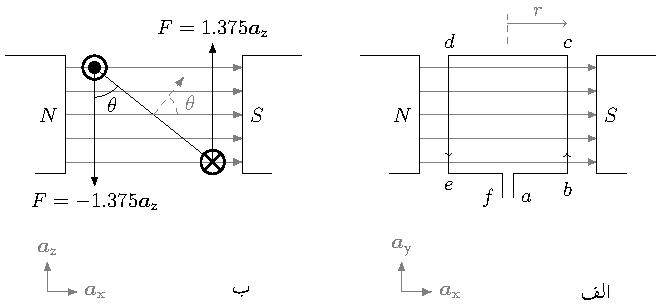
\includegraphics{figEnergyConversionTorqueOnOneTurn}
\begin{tikzpicture}
%grid
%\draw[gray,thick] (-0.5,-0.5) grid (2,2);
%\draw[gray,thin,xstep=0.1,ystep=0.1] (-0.5,-0.5) grid (2,2);
\pgfmathsetmacro{\rad}{1}
 \pgfmathsetmacro{\len}{2}
\pgfmathsetmacro{\gap}{0.5}
%defining mid point arrow macros
\tikzset{->-/.style={decoration={
  markings,
  mark=at position #1 with {\arrow{>}}},postaction={decorate}}}
\tikzset{-<-/.style={decoration={
  markings,
  mark=at position #1 with {\arrow{<}}},postaction={decorate}}}
%
%flux
\foreach \y in {0.1,0.3,0.5,0.7,0.9}{
\draw[gray,thin,-latex](-\rad-\gap,\y*\len)--(\rad+\gap,\y*\len);
}
%coil as Dot and Cross
\draw[thick](\rad,0.7*\len)node[above left]{$b$} circle (0.2);
\draw[thick](\rad,0.7*\len)++(-135:0.2)--++(45:0.4);
\draw[thick](\rad,0.7*\len)++(135:0.2)--++(-45:0.4);
\draw[thick](-\rad,0.3*\len)node[below right]{$e$} circle (0.2);
\draw[fill](-\rad,0.3*\len) circle (0.1);
%torque and moment arm
\draw[-latex](\rad,0.7*\len)coordinate (kCross)--++(0,-\len)node[below]{$F_{bc}=-1.375 \az $};
\draw[-latex](-\rad,0.3*\len) coordinate(kDot)--++(0,\len)node [above]{$F_{de}=1.375 \az $};
\draw(\rad,0.7*\len)--(-\rad,0.3*\len)coordinate [pos=0.5](kO);
%perpendicular
%\draw[gray,dashed,-latex] (kO)--($(kO)!0.8cm!90:(\rad,0.9*\len)$)coordinate [pos=0.5](kA);
%angle
\draw([shift={(90:0.5)}]-\rad,0.3*\len) arc (90:20:0.5);
\draw(-\rad,0.3*\len)++(55:0.7)node[]{$\theta$};
%magnet
\draw(-\rad-2*\gap,0)--++(1*\gap,0)--++(0,\len)node[left,pos=0.5]{$N$}--++(-\rad,0);
\draw(\rad+2*\gap,0)--++(-1*\gap,0)--++(0,\len)node[right,pos=0.5]{$S$}--++(\rad,0);
%unit vectors
\draw[-latex,gray](-1.8,-2)--++(0.5,0)node[right]{$\ax$};
\draw[-latex,gray](-1.8,-2)--++(0,0.5)node[above]{$\az$};
\draw node at (1.5,-2){ب};
%
%
\begin{scope}[xshift=6cm]
%flux
\foreach \y in {0.1,0.3,0.5,0.7,0.9}{
\draw[gray,thin,-latex](-\rad-\gap,\y*\len)--(\rad+\gap,\y*\len);
}
%coil top view
\draw [->-=0.192,->-=0.815] (0.1,-0.4)node[right]{$a$}--++(0,0.4)--++(\rad-0.1,0)node[below]{$b$}--++(0,\len)node[above]{$c$}--++(-2*\rad,0)node[above]{$d$}--++(0,-\len)node[below]{$e$}--++(\rad-0.1,0)--++(0,-0.4)node[left]{$f$};
\draw[gray,dashed] (0,1.1*\len)--++(0,0.5); 
\draw[gray,->] (0,1.1*\len+0.35)--++(\rad,0)node[above,pos=0.5]{$r$};
%magnet
\draw(-\rad-2*\gap,0)--++(1*\gap,0)--++(0,\len)node[left,pos=0.5]{$N$}--++(-\rad,0);
\draw(\rad+2*\gap,0)--++(-1*\gap,0)--++(0,\len)node[right,pos=0.5]{$S$}--++(\rad,0);
%unit vectors
\draw[-latex,gray](-1.8,-2)--++(0.5,0)node[right]{$\ax$};
\draw[-latex,gray](-1.8,-2)--++(0,0.5)node[above]{$\ay$};
\draw node at (1.5,-2){الف};
%
\end{scope}
\end{tikzpicture}%
\caption{ایک چکر کے لچھے پر قوت اور قوت مروڑ}
\label{شکل_تبادلہ_طاقت_لچھے_پر_قوت_اور_مروڑ}
\end{figure}
%
حل:\quad
شکل-الف اور ب میں کارتیسی اکائی سمتیات دکھائے  گئے ہیں۔برقی تار کے سروں کو نظر انداز کرتے ہوئے  اسے ایک بند مستطیل تصور کرتے ہیں۔ یوں   شکل-الف میں  برقی رو کے رخ تار کے اطراف کی سمتی لمبائیاں  درج ذیل ہوں گی جہاں \عددی{l} محوری لمبائی ہے
\begin{align*}
\kvec{L}_{bc}&=l \ay\\
\kvec{L}_{cd}&=-2 r \ax\\
\kvec{L}_{de}&=-l \ay\\
\kvec{L}_{eb}&=2 r \ax
\end{align*}
 جبکہ \عددیء{\kvec{B}=B_0 \ax} ہو گا۔ ان میں \عددی{\ax} اور \عددی{\ay} اکائی سمتیات ہیں۔یوں مساوات \حوالہ{مساوات_تبادلہ_قوت_رو}  کے تحت ان اطراف پر قوت (نیوٹن) درج ذیل ہو گی۔
\begin{align*}
\kvec{F}_{bc}&= i \left(\kvec{L}_{bc} \times B_0 \ax \right)\\
&=5 \left(0.5 \ay \times 0.55 \ax \right)\\
&=-1.375 \az\\
\kvec{F}_{cd}&= 5\left(-0.3\ax \times 0.55 \ax \right)\\
&=0\\
\kvec{F}_{de}&= 5 \left(-0.5\ay \times 0.55 \ax \right)\\
&=1.375 \az\\
\kvec{F}_{eb}&= 0
\end{align*}
ہم دیکھتے ہیں کہ  صرف محوری  اطراف پر قوتیں  پائی جاتی  ہیں جنہیں شکل \حوالہ{شکل_تبادلہ_طاقت_لچھے_پر_قوت_اور_مروڑ}-ب  میں دکھایا گیا ہے۔شکل \حوالہ{شکل_تبادلہ_طاقت_لچھے_پر_قوت_اور_مروڑ}-الف اور ب میں \عددی{b} اور \عددی{e} کے بیچ فاصلہ \عددی{2r} ہے۔محوری اطراف پر اثر انداز قوت، مروڑ پیدا کرتی ہیں جس کا رخ  دائیں ہاتھ کے قانون سے حاصل ہو گا۔مستطیل تار پر قوت مروڑ (نیوٹن میٹر)  درج ذیل ہو گا۔
\begin{align*}
\kvec{\tau}&=(1.375)( 2)( 0.15)( \sin \theta) \ay\\
&=0.4125 \sin \theta \ay
\end{align*}
\انتہا{مثال}
%

مساوات \حوالہ{مساوات_تبادلہ_برقی_میدان_قوت} تا مساوات \حوالہ{مساوات_تبادلہ_توانائی_لورینز} کا استعمال صرف سادہ ترین صورتوں میں ممکن ہوتا ہے۔ حقیقی  مشینوں میں ان مساوات سے قوت  تعین کرنا مشکل ثابت ہوتا ہے۔ آئیں  ایک ایسی ترکیب  سیکھتے ہیں جس سے ہم  مختلف مشینوں میں پائی جانی والی  قوتیں  تعین کر سکیں ۔ اس ترکیب کا نام\اصطلاح{  ہم توانائی}\فرہنگ{ہم توانائی}\حاشیہب{co-energy}\فرہنگ{co-energy} ہے  جو توانائی کے اٹل ہونے پر مبنی ہے۔

گھومتی برقی مشین عموماً دو لچھوں پر مشتمل ہوتی ہیں۔ ان میں ایک لچھا  مشین کے ساکن حصہ پر لپٹا ہوتا ہے جس کی بنا یہ ساکن رہتا ہے اور \اصطلاح{ساکن لچھا}\فرہنگ{ساکن لچھا}\فرہنگ{لچھا! ساکن}\حاشیہب{stator coil}\فرہنگ{stator coil}   کہلاتا ہے ۔  دوسرا لچھا  مشین کے گھومتے   حصہ پر لپٹا ہوتا ہے اور مشین گھومنے سے یہ بھی گھومتا ہے۔ اس کو \اصطلاح{گھومتا لچھا}\فرہنگ{گھومتا لچھا}\فرہنگ{لچھا!گھومتا}\حاشیہب{rotor coil}\فرہنگ{rotor coil}  کہتے ہیں۔ان  لچھوں کو دو عدد مقناطیس تصور کرتے ہوئے ایسی مشینوں کی کارکردگی  باآسانی  سمجھی جا سکتی ہے۔

 جس طرح دو مقناطیس اگر قریب لائے جائیں تو یہ کوشش کرتے ہیں کہ ایک کا شمال \عددیء{N} دوسرے کے جنوب \عددیء{S} کی سمت  ہو۔

 موٹر کے دو  لچھے مقناطیس پیدا کرتے ہیں۔ہم جانتے ہیں کہ  ایک مقناطیس  کے شمال \عددیء{N} اور دوسرے کے جنوب \عددیء{S} کے بیچ قوت کشش پائی جاتی ہے۔ ساکن لچھے کا مقناطیسی بہاو  گھومتے لچھے کے مقناطیسی بہاو سے کچھ آگے رہ کر اسے کھینچ  کر  کام کرتا ہے۔ جنریٹر میں اس کے برعکس  گھومتا لچھا، ساکن لچھے پر کام کرتے ہوئے اس میں برقی دباو پیدا کرتا ہے۔

توانائی کے طریقے کو شکل \حوالہ{شکل_تبادلہ_توانائی_نظام_بطور_ڈبہ}  کی مدد سے سمجھا جا سکتا ہے۔یہاں مقناطیسی نظام کو ایک ڈبہ  مانند دکھایا گیا ہے۔ اس نظام کو برقی توانائی مہیا کی جاتی ہے جس کو یہ میکانی توانائی میں تبدیل کرتا ہے۔ یہاں برقی توانائی کے متغیرات  \عددیء{e} اور \عددیء{i} ہیں جبکہ میکانی توانائی کے متغیرات فاصلہ \عددیء{x} اور میدانی قوت\حاشیہد{میدانی قوت \عددیء{F_m} میں چھوٹی لکھائی میں \عددیء{m} لفظ میدانی کو ظاہر کر رہا ہے۔} \عددیء{F_m} ہیں۔ اس شکل میں بائیں یعنی ابتدائی یا اولین جانب \عددیء{i} کا رُخ باہر سے اندر ہے جبکہ  دائیں یعنی ثانوی جانب  \عددیء{F_m} کا رُخ اندر سے  باہر رخ ہے۔یہ  ٹرانسفارمر دور کے شکل \حوالہ{شکل_ٹرانسفارمر_کامل_بار_بردار_ٹرانسفارمر}  کی مانند ہے۔

جہاں نظام میں توانائی کے ضیاع کو ذخیرہ توانائی سے علیحدہ کرنا ممکن ہو  وہاں توانائی کے ضیاع  کو بیرونی رکن تصور  کیا جاتا ہے۔ شکل \حوالہ{شکل_تبادلہ_توانائی_قوت_پیدا_کرتا_آلا}   میں ایک ایسا ہی نظام دکھایا گیا ہے جس میں  لچھا برقی نظام  اور حرکی حصہ میکانی نظام کو ظاہر کرتے ہیں اور  لچھے میں توانائی کے ضیاع کو بیرونی  مزاحمت \عددیء{R} سے ظاہر کیا گیا ہے۔
\begin{figure}
\centering
%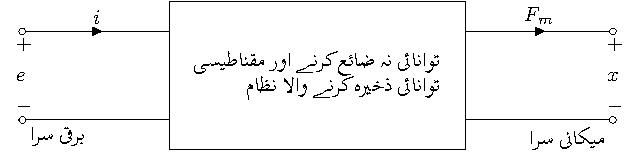
\includegraphics{figEnergyConversionBasicBlockDiagram}
\begin{tikzpicture}
%grid
%\draw[gray,thick] (0,0) grid (5,5);
%\draw[gray,thin,xstep=0.1,ystep=0.1] (0,0) grid (5,5);
\pgfmathsetmacro{\l}{5}
 \pgfmathsetmacro{\b}{2.5}
\draw (0,0)coordinate(a){}--++(0:\l)coordinate(b){}--++(90:\b)coordinate(c){}--++(180:\l)coordinate(d){}--cycle;
\draw($(a)!0.2!(d)$) to [short,-o]++(180:\b)coordinate(leftLow){};
\draw($(a)!0.8!(d)$) to [short,-o,i_<={$i$}]++(180:\b)coordinate(leftUpper){};
\draw($(b)!0.2!(c)$) to [short,-o]++(0:\b)coordinate(rightLow){};
\draw($(b)!0.8!(c)$) to [short,-o,i={$F_m$}]++(0:\b)coordinate(rightUpper){};
%
\node[below right] at (leftLow){\RL{برقی سرا}};
\node[below left] at (rightLow){\RL{میکانی سرا}};
\node[ align=right] at (0.5*\l,0.5*\b) {\RL{توانائی نہ ضائع کرنے  اور مقناطیسی} \\ \RL{توانائی ذخیرہ کرنے والا نظام}};
\draw node at ($(leftLow) ! 0.5! (leftUpper)$){$
\begin{aligned}
&+\\
&e\\
&-
\end{aligned}
$};
%
\draw node at ($(rightLow) ! 0.5! (rightUpper)$){$
\begin{aligned}
&+\\
&x\\
&-
\end{aligned}
$};
\end{tikzpicture}%
\caption{ برقی توانائی سے میکانی توانائی کے تبادلہ کا نظام۔}
\label{شکل_تبادلہ_توانائی_نظام_بطور_ڈبہ}
\end{figure}
%
\begin{figure}
\centering
%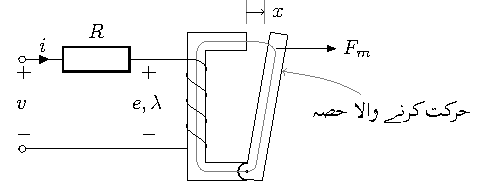
\includegraphics{figEnergyConversionForceGeneratingDevice}
\begin{tikzpicture}
%grid
%\draw[gray,thick] (-2,-2) grid (2,2);
%\draw[gray,thin,xstep=0.1,ystep=0.1] (-2,-2) grid (2,2);
\pgfmathsetmacro{\h}{2.5}
 \pgfmathsetmacro{\w}{1}
\pgfmathsetmacro{\t}{0.3}
\pgfmathsetmacro{\N}{4}
 \pgfmathsetmacro{\r}{\t/2}
\pgfmathsetmacro{\g}{0.3}   %gap between coil and edge of window
%coil step
\pgfmathsetmacro{\stepHL}{(\h-2*\t-2*\g)/(\N-1)}
\draw ([shift=(90:\r)]0,0) arc (90:270:\r)--++(180:\w)--++(90:\h)--++(0:\w)--++(270:\t)--++(180:\w-\t)--++(270:\h-2*\t)--++(0:\w-\t);
\draw ([shift=(90:0.9*\r)]0,0)coordinate(pivotUpper){} arc (90:270:0.9*\r)coordinate(pivotLower){};
\draw(pivotUpper)--++(0:0.01)coordinate(leverLowerL){}--++(80:\h-0.8*\t)coordinate(leverUpperL){}--++(-10:\t)coordinate(leverUpperR){}--++(-100:\h)coordinate(leverLowerR){}--(pivotLower);
%
\coordinate  (kL) at ($(leverLowerL) ! 0.85 ! (leverUpperL)$);
\coordinate (kR) at ($(leverLowerR) ! 0.85 ! (leverUpperR)$);
\coordinate (kM) at ($(kL) ! 0.5 ! (kR)$);


\path[gray] (0,0)--++(180:\w-0.5*\t)coordinate[pos=0.8](kDashA)--++(90:\h-\t)coordinate[pos=0.1](kDashB)coordinate[pos=0.9](kDashC)--++(0:\w-0.5*\t)coordinate[pos=0.2](kDashD)coordinate[pos=0.9](kDashE) to [out=0,in=90] (kM)--++(-100:\h-2*\t) to [out=-100,in=0] (0,0);
%
\draw[gray](0,0)--(kDashA) to [out=180,in=-90] (kDashB)--(kDashC) to [out=90,in=180](kDashD) --(kDashE) to [out=0,in=90] (kM)--++(-100:\h-2*\t) to [out=-100,in=0] (0,0);
\draw[solid] (0,0) circle (0.5 pt);   %mark centre of pivot
\draw[-latex]  (kM)++(80:0.1) -- ++(0:1)node[right]{$F_m$};
%
\draw[gray](0,\h)--++(90:0.4)coordinate[pos=0.5](distanceL);
\draw[gray](0,\h)++(0.3,0)--++(90:0.4)coordinate[pos=0.5](distanceR);
\draw[->](distanceL)--(distanceR)node[right]{$x$};
%COIL
\def\leftEdge{-\w};
\def\coilTop{\h-\t-\g};
%
\draw(\leftEdge+\t/4,\coilTop) to [out=0,in=45] (\leftEdge+\t,{\coilTop-\stepHL/2}); %top half section
%coil itself
\pgfmathsetmacro{\nLend}{\N-2}
\foreach \y in { 0, ..., \nLend }{
\draw (\leftEdge,{\coilTop-\stepHL/2-\y*\stepHL}) to [out=-135,in=45] (\leftEdge+\t,{\coilTop-\stepHL/2-\y*\stepHL-\stepHL});
} 
%left hand terminals
\draw (\leftEdge+\t/4,\coilTop)--++(-1.25*\t,0) node(TA){};
\draw (\leftEdge,\coilTop-\N*\stepHL+0.5*\stepHL)--++(-1*\t,0)node(TB){};
%--------------------
\draw (TA) to [european resistor,i_<={$i$},-o,l_={$R$}]++(180:2.5)coordinate(supplyP);
\draw (TB) to [short,-o]++(180:2.5)coordinate(supplyN);
\node at ($(supplyP)!0.5!(supplyN)$){$\begin{aligned} &+\\&v\\&-  \end{aligned}$};
%text
\node[left] at ($(TA)!0.5!(TB)$){$\begin{aligned} &+\\e&,\lambda\\&-  \end{aligned}$};
\node[right](urdu) at (1,1){\RL{حرکی حصہ}};
\draw[gray,<-](0.6,1.7) to [out=-10,in=150] (urdu);
%
\end{tikzpicture}%

\caption{ قوت پیدا کرنے والا آلا۔}
\label{شکل_تبادلہ_توانائی_قوت_پیدا_کرتا_آلا}
\end{figure}

توانائی کا بنیادی اصول کہتا ہے کہ توانائی نا تو پیدا کی جا سکتی ہے اور نا ہی اسے تباہ کیا جا سکتا ہے۔ اس کو صرف ایک قسم  سے دوسرے قسم کی توانائی میں تبدیل کیا جا سکتا ہے۔ یوں نظام کو فراہم برقی توانائی \عددیء{\partial W_{\textup{برقی}}} کا ایک حصہ میکانی توانائی \عددیء{\partial W_{\textup{میکانی}}}  میں تبدیل ہو گا جبکہ اس کا دوسرا حصہ، \عددیء{\partial W_{\textup{مقناطیسی}}}،  مقناطیسی میدان میں  ذخیرہ ہو گا  اور باقی حصہ،\عددیء{\partial W_{\textup{ضائع}}}،  مختلف طریقوں سے  ضائع  ہو گیا جو ہمارے کسی کام نہ آ سکے گا:
\begin{align}
\partial W_{\textup{برقی}}=\partial W_{\textup{میکانی}}+\partial W_{\textup{مقناطیسی}}+\partial W_{\textup{ضائع}}
\end{align}
برقی توانائی کے ضیاع کو نظرانداز کرتے ہوئے 
\begin{align}
\partial W_{\textup{برقی}}=\partial W_{\textup{میکانی}}+\partial W_{\textup{مقناطیسی}}
\end{align}
لکھا جا سکتا ہے جس  کو \عددیء{\partial t} سے تقسیم کر کے

\begin{align}
\frac{\partial W_{\textup{برقی}}}{\partial t}=\frac{\partial W_{\textup{میکانی}}}{\partial t}+\frac{\partial W_{\textup{مقناطیسی}}}{\partial t}
\end{align}
لکھا جا سکتا ہے جو توانائی کی بجائے طاقت کی بات کرتی ہے۔ اس مساوات کے  بائیں ہاتھ  برقی طاقت کو \عددیء{e i}  اور  دائیں ہاتھ میکانی حصہ میں \عددیء{\partial W_{\textup{میکانی}}=F_m \partial x} لکھ کر
\begin{align}
e i = F_m \frac{\partial x}{\partial t} +\frac{\partial W_m}{\partial t}
\end{align}
حاصل ہو گا جہاں \عددیء{W_{\textup{مقناطیسی}}}  کو \عددیء{W_m} لکھا گیا ہے۔مساوات \حوالہ{مساوات_مقناطیسی_دور_فیراڈے_قانون}   استعمال کرتے ہوئے اس کو 
\begin{align}
i \frac{\partial \lambda}{\partial t}=F_m \frac{\partial x}{\partial t}+\frac{\partial W_m}{\partial t}
\end{align}
لکھا جا سکتا ہے۔دونوں اطراف کو \عددی{\partial t} سے ضرب دے کر ترتیب نو کرتے  ہوئے درج ذیل حاصل ہو گا۔
\begin{align}\label{مساوات_برقی_مقناطیسی_تبادلہ_توانائی_کا_طریقہ}
\partial W_m=i \partial \lambda-F_m \partial x
\end{align}
مساوات \حوالہ{مساوات_برقی_مقناطیسی_تبادلہ_توانائی_کا_طریقہ} توانائی کے طریقہ کی بنیاد ہے۔ اس مساوات کو استعمال کرتے وقت یاد رہے کہ قوت بنیادی طور پر لورینز کے قانون\حاشیہب{Lorenz equation} سے ہی پیدا ہوتی ہے۔مساوات \حوالہ{مساوات_برقی_مقناطیسی_تبادلہ_توانائی_کا_طریقہ}  میں برقی متغیرات \عددیء{i} اور \عددیء{e} کی بجائے \عددیء{i} اور \عددیء{\lambda} ہیں۔ لہٰذا شکل \حوالہ{شکل_تبادلہ_توانائی_نظام_بطور_ڈبہ}    کو شکل \حوالہ{شکل_تبادلہ_توانائی_قوت_پیدا_کرتا_آلا_زیادہ_معلومات}   کی طرح بھی بنایا جا سکتا ہے۔
\begin{figure}
\centering
%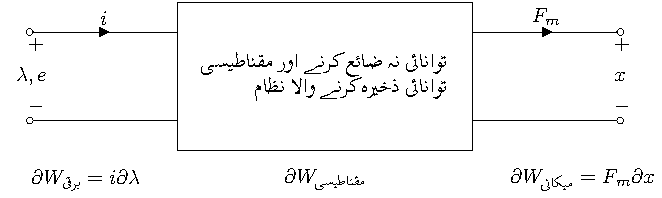
\includegraphics{figEnergyConversionBasicBlockDiagramDetailed}
\begin{tikzpicture}
%grid
%\draw[gray,thick] (0,0) grid (5,5);
%\draw[gray,thin,xstep=0.1,ystep=0.1] (0,0) grid (5,5);
\pgfmathsetmacro{\l}{5}
 \pgfmathsetmacro{\b}{2.5}
\draw (0,0)coordinate(a){}--++(0:\l)coordinate(b){}--++(90:\b)coordinate(c){}--++(180:\l)coordinate(d){}--cycle;
\draw($(a)!0.2!(d)$) to [short,-o]++(180:\b)coordinate(leftLow){};
\draw($(a)!0.8!(d)$) to [short,-o,i_<={$i$}]++(180:\b)coordinate(leftUpper){};
\draw($(b)!0.2!(c)$) to [short,-o]++(0:\b)coordinate(rightLow){};
\draw($(b)!0.8!(c)$) to [short,-o,i={$F_m$}]++(0:\b)coordinate(rightUpper){};
%
\node[left] at (-0.5,-0.5){$\partial W_{\textup{برقی}}=i \partial \lambda$};
\node[right] at (5.5,-0.5){$\partial W_{\textup{میکانی}}=F_m \partial x$};
\node at (2.5,-0.5){$\partial W_{\textup{مقناطیسی}}$};
\node[ align=right] at (0.5*\l,0.5*\b) {\RL{توانائی نہ ضائع کرنے  اور مقناطیسی} \\ \RL{توانائی ذخیرہ کرنے والا نظام}};
%
\draw node at ($(leftLow) ! 0.5! (leftUpper)$){$
\begin{aligned}
&+\\
\lambda&,e\\
&-
\end{aligned}
$};
%
\draw node at ($(rightLow) ! 0.5! (rightUpper)$){$
\begin{aligned}
&+\\
&x\\
&-
\end{aligned}
$};
\end{tikzpicture}%

\caption{توانائی کی قسم تبدیل کرنے والا ایک نظام۔}
\label{شکل_تبادلہ_توانائی_قوت_پیدا_کرتا_آلا_زیادہ_معلومات}
\end{figure}

کسی بھی تفاعل\حاشیہب{function} \عددیء{z(x,y)} کا کل تفرق درج ذیل ہو گا جہاں \عددی{\frac{\partial z}{\partial x} } لیتے ہوئے \عددی{y} کو مستقل تصور کیا جاتا ہے اور \عددی{\frac{\partial z}{\partial y}} لیتے ہوئے \عددی{x} کو مستقل تصور کیا جاتا ہے۔
\begin{align}\label{مساوات_تبادلہ_جزوی_تفرق_عمومی_الف}
\partial z(x,y)=\frac{\partial z}{\partial x} \dif x+\frac{\partial z}{\partial y} \dif y
\end{align}
اسی طرح \عددیء{W_m(x,\lambda)} کا کل تفرق
\begin{align}\label{مساوات_تبادلہ_جزوی_تفرق_عمومی_ب}
\partial W_m(x,\lambda)=\frac{\partial W_m}{\partial x}\dif x+\frac{\partial W_m}{\partial \lambda}\dif \lambda
\end{align}
ہو گا جس کا موازنہ مساوات \حوالہ{مساوات_برقی_مقناطیسی_تبادلہ_توانائی_کا_طریقہ} کے ساتھ کر کے درج ذیل اخذ  کیا جا سکتا ہے جہاں ایک متغیر کے ساتھ جزوی تفرق لیتے وقت دوسرے متغیر  کو صریحاً مستقل ظاہر کیا گیا ہے۔
\begin{align}
F_m(x,\lambda)&=-\left. \frac{\partial W_m(x,\lambda)}{\partial x}\right|_{\lambda_0}\label{مساوات_تبادلہ_توانائی_قوت_برقی_رو}\\
i(x,\lambda)&=\left. \frac{\partial W_m(x,\lambda)}{\partial \lambda}\right|_{x_0}\label{مساوات_تبادلہ_توانائی_سے_رو}
\end{align}
مقناطیسی میدان میں مقناطیسی توانائی \عددیء{W_m(x,\lambda)} دریافت کر کے مساوات \حوالہ{مساوات_تبادلہ_توانائی_قوت_برقی_رو}  کی  استعمال سے قوت  دریافت کی جا سکتی ہے۔شکل \حوالہ{شکل_تبادلہ_توانائی_قوت_پیدا_کرتا_آلا} میں قوت اور خلائی درز میں مقناطیسی بہاو ایک دوسرے کے متوازی ہیں۔ اگلے حصہ میں مقناطیسی توانائی کا حصول سکھایا جائے گا۔

\حصہ{تبادلہ توانائی والا ایک لچھے کا نظام}
شکل \حوالہ{شکل_تبادلہ_توانائی_قوت_پیدا_کرتا_آلا}  میں  ایک لچھے کا سادہ نظام دکھایا گیا ہے۔ لچھے میں برقی ضیاع کو بیرونی مزاحمت سے ظاہر کیا گیا ہے جبکہ میکانی نظام میں حرکی حصہ کی کمیت کو نظرانداز کیا گیا ہے۔ جہاں اس کمیت  کا اثر جاننا ضروری ہو وہاں  اس کو ایک بیرونی کمیت تصور کیا جا سکتا ہے۔ اس طرح تبادلہ توانائی کے نظام پر غور کرنا آسان ہوتا ہے۔ 

قوت پیدا کرنے والی مشین میں حرکت ناگزیر ہے۔عموماً حرکت تب ممکن ہو گی جب مقناطیسی قالب میں قابل تبدیل خلاء موجود ہو۔ قالب میں خلاء کی موجودگی کی بنا عام طور  پر \عددیء{\Re_a \gg \Re_c} ہو گا اور ایسا  مقناطیسی دور حل کرتے ہوئے \عددیء{\Re_c} کو نظرانداز کیا جائے گا۔یوں، جیسا مساوات \حوالہ{مساوات_مقناطیسی_ڈور_بہاو_مساوی_دباو_بٹا_ہچکچاہٹ}  میں دیا گیا ہے،  مقناطیسی دباو \عددیء{\tau} اور مقناطیسی بہاو \عددیء{\phi}  براہ راست متناسب ہوں گے۔ ایسی صورت میں مساوات \حوالہ{مساوات_مقناطیسی_دور_خود_امالہ_تعریف}  میں  امالہ \عددی{L} شکل \حوالہ{شکل_تبادلہ_توانائی_قوت_پیدا_کرتا_آلا}   میں خلاء کی لمبائی \عددیء{x}  پر منحصر ہو گی لہٰذا اس مساوات کو درج ذیل لکھتے ہیں۔
\begin{align}\label{مساوات_تبادلہ_ارتباط_بہاو_اور_امالہ}
\lambda=L(x) i
\end{align}

شکل \حوالہ{شکل_تبادلہ_توانائی_قوت_پیدا_کرتا_آلا}  میں قوت \عددیء{F_m}  کے رخ طے ہونے والا فاصلہ \عددیء{x} ہے۔ یوں  میکانی کام \عددیء{\partial W_{\textup{میکانی}}=F_m \dif x} ہو گا جبکہ  فراہم برقی توانائی \عددیء{\partial W_{\textup{برقی}}=i \dif \lambda} ہو گی۔ یوں شکل \حوالہ{شکل_تبادلہ_توانائی_قوت_پیدا_کرتا_آلا}   کو مساوات \حوالہ{مساوات_برقی_مقناطیسی_تبادلہ_توانائی_کا_طریقہ}  ظاہر کرتی ہے۔ مقناطیسی میدان میں ذخیرہ توانائی \عددیء{W_m} کو مساوات \حوالہ{مساوات_برقی_مقناطیسی_تبادلہ_توانائی_کا_طریقہ}  کا تکمل\حاشیہب{integral}  لے کر حاصل کرتے ہیں۔
\begin{align}\label{مساوات_تبادلہ_توانائی_تکمل}
\int \partial W_m(x,\lambda) = \int i(x,\lambda) \dif \lambda-\int F_m(x,\lambda) \dif x
\end{align}
اس تکمل کا حصول شکل \حوالہ{شکل_تبادلہ_توانائی_مقناطیسی_میدان_میں_توانائی}   سے واضح ہو گا۔ابتدائی نقطے پر مقناطیسی نظام کو کوئی برقی توانائی فراہم نہیں کی گئی ہے۔یوں نظام میں  برقی رو صفر ہو گی جس کی بنا  مقناطیسی بہاو اور  ارتباط بہاو بھی صفر ہوں گے  لہٰذا  مقناطیسی میدان میں مقناطیسی توانائی بھی صفر ہو گی۔ کسی بھی مقناطیس کی قوت کشش اس کی مقناطیسی بہاو پر منحصر ہوتی ہے لہٰذا صفر مقناطیسی بہاو کی بنا اس نظام میں قوت کشش صفر ہو گا اور یوں اس میں حرکت بھی صفر ہو گا۔اس طرح ابتدائی نقطہ پر درج ذیل ہوں گے۔
\begin{align*}
i=\phi=\lambda=W_m=F_m=x=0
\end{align*}

ابتدائی نقطہ شکل \حوالہ{شکل_تبادلہ_توانائی_مقناطیسی_میدان_میں_توانائی}  میں دکھایا گیا ہے۔ اب لچھے کو برقی توانائی فراہم کی جاتی ہے۔ لچھے میں برقی رو کی بنا قوت اور حرکت پیدا ہو گی۔  آخر کار  نظام اختتامی نقطے پر پہنچے گا۔اختتامی نقطہ بھی شکل میں دکھایا گیا ہے۔ اس نقطہ پر \عددیء{\lambda=\lambda_0} اور \عددیء{x=x_0} ہیں اور  مقناطیسی میدان میں توانائی \عددیء{W_m(x_0,\lambda_0)} ہے۔ابتدائی نقطہ  سے اختتامی نقطہ  تک پہنچنے کے لئے  برقی توانائی کو یوں بڑھایا جاتا ہے  کہ \عددیء{\lambda} اور \عددیء{x}  شکل \حوالہ{شکل_تبادلہ_توانائی_مقناطیسی_میدان_میں_توانائی}  میں موٹی لکیر  (اصل راستے) پر رہیں۔ آخری نقطہ پر مقناطیسی میدان میں مقناطیسی توانائی \عددیء{W_m(x_0,\lambda_0)} جاننے  کے لئے اصل راستے پر  مساوات \حوالہ{مساوات_تبادلہ_توانائی_تکمل}  کا تکمل حاصل کرنا  ہو گا جو ایک مشکل کام ہے۔اس راہ پر تکمل کی بجائے ہم متبادل راستہ اختیار کرتے ہیں۔
\begin{figure}
\centering
%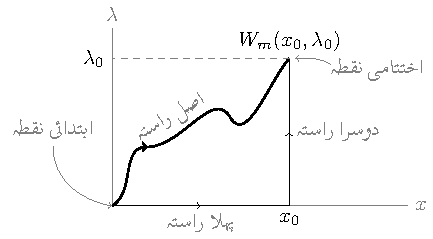
\includegraphics{figEnergyConversionEnergyInMagneticField}
\begin{tikzpicture}
%grid
%\draw[gray,thick] (0,0) grid (5,5);
%\draw[gray,thin,xstep=0.1,ystep=0.1] (0,0) grid (5,5);
\pgfmathsetmacro{\l}{5}
 \pgfmathsetmacro{\b}{2.5}
\draw[](0,0)--(5,0)node[ right]{$x$};
\draw[](0,0)--(0,3)node[above]{$\lambda$};
%ACTUAL PATH
\draw[thick,->] (0,0) to [out=30,in=180] (0.6,1);
\draw[thick] (0.6,1) to [out=0,in=120] (2,1.5) to [out=-60,in=-130](3,2.5) ;
%EASY PATHS
\draw[->](0,0)--(1.5,0)node[,below]{\RL{پہلی راہ}};
\draw(1.5,0)--(3,0)node[below]{$x_0$};
\draw[->](3,0)--(3,1.25)node[,right]{\RL{دوسری راہ}};
\draw(3,1.25)--(3,2.5) node [above]{$W_m(x_0,\lambda_0)$};
\node[,rotate=30] at (1,1.5){\RL{اصل راہ}};
\draw[,dashed](3,2.5)--(0,2.5);
\node[left] at (0,2.5){$\lambda_0$};
%text
\node[,above] at (-1,1){\RL{ابتدائی نقطہ}};
\draw[,<-](0,0) to [out=170,in=-90] (-1,1);
\node[,above] at (4.5,2){\RL{اختتامی  نقطہ}};
\draw[,<-](3.1,2.5) to [out=0,in=150] (3.7,2.4);
\end{tikzpicture}%
\caption{مقناطیسی میدان میں توانائی۔}
\label{شکل_تبادلہ_توانائی_مقناطیسی_میدان_میں_توانائی}
\end{figure}


ہم اس حقیقت سے فائدہ اٹھاتے ہیں کہ مقناطیسی میدان ایک \اصطلاح{قدامت پسند میدان}\فرہنگ{قدامت پسند میدان}\حاشیہب{conservative field}\فرہنگ{conservative field}   ہے جس کا مطلب ہے کہ مقناطیسی میدان میں مقناطیسی توانائی صرف اور صرف اختتامی نقطہ کے \عددیء{x_0} اور \عددیء{\lambda_0} کی مقدار پر منحصر ہو گی\حاشیہد{تجاذبی میدان بھی قدامت پسند میدان ہے۔ اسی لئے اگر کمیت \عددیء{m} کو کسی بھی راستے \عددیء{h} کی بلندی تک لے جایا جائے تو اس کی خفی توانائی \عددیء{mgh} ہو گی۔}۔چونکہ توانائی کا دارومدار راہ پر  منحصر نہیں ہے لہٰذا  توانائی کے حصول کے  تکمل میں ہم من پسند  راستہ اختیار کرتے ہیں ۔ہم تکمل لیتے ہوئے  شکل  \حوالہ{شکل_تبادلہ_توانائی_مقناطیسی_میدان_میں_توانائی} میں ابتدائی نقطہ سے  پہلی راہ چل کر  فاصلہ  \عددیء{x_0} طے کر کے  دوسری راہ اختیار کر کے اختتامی نقطہ \عددیء{(x_0,\lambda_0)} تک پہنچتے ہیں۔ یوں مساوات \حوالہ{مساوات_تبادلہ_توانائی_تکمل}   کو دو تکملات کا مجموعہ  لکھا جائے گا۔ایک تکمل نقطہ \عددیء{(0,0)} سے نقطہ  \عددیء{(x_0,0)} تک اور دوسرا یہاں سے  نقطہ \عددیء{(x_0,\lambda_0)}  تک لیا جائے گا:
\begin{align}\label{مساوات_تبادلہ_توانائی_تکمل_راستہ_دو_ٹکڑے}
\int\limits_{\text{\RL{اصل راہ}}} \partial W_m(x,\lambda) =\int\limits_{\text{\RL{پہلی راہ}}} \partial W_m(x,\lambda) +\int\limits_{\text{\RL{دوسری راہ}}} \partial W_m (x,\lambda)
\end{align}
اس مساوات کے دائیں ہاتھ تکملات کو باری باری دیکھتے ہیں۔پہلی راہ تکمل کو مساوات \حوالہ{مساوات_تبادلہ_توانائی_تکمل} کی مدد سے لکھتے ہیں۔
\begin{align}\label{مساوات_تبادلہ_توانائی_تکمل_پہلا_راستہ}
\int\limits_{\text{\RL{پہلی راہ}}} \partial W_m(x,\lambda) =\int_0^0 i(x,0) \dif \lambda-\int_0^{x_0} F_m(x,0) \dif x
\end{align}


جیسا  شکل \حوالہ{شکل_تبادلہ_توانائی_مقناطیسی_میدان_میں_توانائی}  میں دکھایا گیا ہے، پہلی راہ پر  \عددیء{\lambda=0} ہے۔ مساوات \حوالہ{مساوات_تبادلہ_توانائی_تکمل_پہلا_راستہ}  میں اس بات کو برقی رو \عددیء{i(x,0)}  اور قوت \عددیء{F_m(x,0)}  لکھ کر واضح کیا گیا ہے۔ چونکہ ابتدائی اور اختتامی نقطوں پر \عددیء{\lambda} صفر ہے  لہٰذا  \عددیء{\int_0^0 i(x,0)\dif \lambda =0} ہو گا۔ ایسے تکمل کی قیمت صفر ہوتی ہے  جس کا ابتدائی اور اختتامی نقطے ایک دوسرے کے برابر ہوں۔

 پہلی راہ پر \عددیء{\lambda=0} ہونے کی بنا اس راہ پر  مقناطیسی بہاو بھی صفر ہو گا لہٰذا اس راہ  پر  مقناطیسی اثر  نہیں پایا جائے گا اور  قوت \عددیء{F_m} صفر ہو گا۔ ہم جانتے ہیں کہ صفر کا تکمل صفر  ہوتا ہے لہٰذا  \عددیء{\int_0^{x_0} F_m(x,0)\dif x=0} ہو گا۔ یوں پہلی راہ پر  کا تکمل (مساوات \حوالہ{مساوات_تبادلہ_توانائی_تکمل_پہلا_راستہ}) صفر ہو گا:
\begin{align}
\int\limits_{\text{\RL{پہلی راہ}}} \partial W_m(x,0) =\int_0^0 i(x,0) \dif \lambda-\int_0^{x_0} F_m(x,0) \dif x=0
\end{align}
مساوات \حوالہ{مساوات_تبادلہ_توانائی_تکمل_راستہ_دو_ٹکڑے} میں  دوسری راہ کا تکمل
\begin{align}\label{مساوات_تبادلہ_دوسری_راہ_قوت_تکمل}
\int\limits_{\text{\RL{دوسری راہ}}} \partial W_m(x_0,\lambda) =\int_0^{\lambda_0} i(x_0,\lambda) \dif \lambda-\int_{x_0}^{x_0} F_m(x_0,\lambda) \dif x
\end{align}
ہو گا۔دوسری راہ پر  \عددیء{x=x_0} ہے لہٰذا مساوات \حوالہ{مساوات_تبادلہ_دوسری_راہ_قوت_تکمل} میں دائیں ہاتھ دوسرے تکمل کا ابتدائی نقطہ \عددی{x_0}  اور اختتامی نقطہ بھی \عددی{x_0} ہو گا جس کی بنا قوت کا تکمل صفر ہو گا:
\begin{align}\label{مساوات_تبادلہ_قوت_تکمل_صفر_ہے}
\int_{x_0}^{x_0} F_m(x_0,\lambda) \dif x=0
\end{align}
آخر میں مساوات \حوالہ{مساوات_تبادلہ_دوسری_راہ_قوت_تکمل} کے دائیں ہاتھ،  برقی رو کا تکمل حل کرنا باقی ہے۔ مساوات \حوالہ{مساوات_تبادلہ_ارتباط_بہاو_اور_امالہ}   استعمال کرتے ہوئے اسے حل کرتے ہیں۔
\begin{align}\label{مساوات_تبادلہ_رو_تکمل_غیر_صفر}
\int_0^{\lambda_0} i(x_0,\lambda) \dif \lambda=\frac{1}{L(x_0)} \int_0^{\lambda_0} \lambda \dif \lambda=\frac{\lambda_0^2}{2 L(x_0)}
\end{align}
مساوات \حوالہ{مساوات_تبادلہ_دوسری_راہ_قوت_تکمل}، مساوات \حوالہ{مساوات_تبادلہ_قوت_تکمل_صفر_ہے} اور مساوات \حوالہ{مساوات_تبادلہ_رو_تکمل_غیر_صفر} کے نتائج استعمال کرتے ہوئے مساوات \حوالہ{مساوات_تبادلہ_توانائی_تکمل_راستہ_دو_ٹکڑے} میں دیے تکمل کا حل لکھتے ہیں:
\begin{align*}
W(x_0,\lambda_0)=\frac{\lambda_0^2}{2 L(x_0)}
\end{align*}
 اس مساوات میں اختتامی نقطہ کو عمومی نقطہ \عددی{(x,\lambda)} لیتے ہوئے درج ذیل  حاصل ہو گا جو   مقناطیسی میدان میں توانائی کی مساوات ہے۔
\begin{align}\label{مساوات_تبادلہ_مقناطیسی_توانائی}
W(x,\lambda)=\frac{\lambda^2}{2 L(x)}
\end{align}
مساوات \حوالہ{مساوات_تبادلہ_مقناطیسی_توانائی} کی مدد سے مساوات \حوالہ{مساوات_تبادلہ_توانائی_قوت_برقی_رو}  کے ذریعہ قوت  \عددیء{F_m(x,\lambda)} اور مساوات \حوالہ{مساوات_تبادلہ_توانائی_سے_رو}  کے ذریعہ برقی رو \عددیء{i(x,\lambda)}  کا حساب اب ممکن ہے۔
%
\ابتدا{مثال}\شناخت{مثال_تبادلہ_توانائی_درز_میں_مقناطیسی_توانائی}
شکل \حوالہ{شکل_تبادلہ_توانائی_حرکت_اور_توانائی}  میں حرکت کرنے والا ایک مقناطیسی نظام دکھایا گیا ہے۔ حرکی اور ساکن حصوں  کے بیچ خلائی درز \عددیء{g} موجود ہے۔ اگر \عددیء{N=500} ،\عددیء{g=\SI{1}{\milli \meter}} ،\عددیء{b=\SI{0.2}{\meter}}، \عددیء{w=\SI{0.4}{\meter}} اور \عددیء{i=\SI{30}{\ampere}} ہوں تب اس خلائی درز میں توانائی \عددیء{W_m} کیا ہو گی؟
\begin{figure}
\centering
%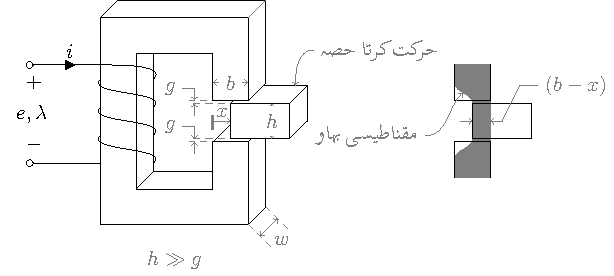
\includegraphics{figEnergyConversionForceOnPlunger}
\begin{tikzpicture}
%grid
%\draw[,thick] (-2,-2) grid (2,2);
%\draw[,thin,xstep=0.1,ystep=0.1] (-2,-2) grid (2,2);
%static section
\pgfmathsetmacro{\h}{3.5}  %height
 \pgfmathsetmacro{\w}{2.5}    %width
\pgfmathsetmacro{\t}{0.6}    %thickness
\pgfmathsetmacro{\dx}{0.3}    %depth-x
\pgfmathsetmacro{\dy}{0.3}    %depth-y
\pgfmathsetmacro{\nL}{4}        %turns on left hand side
 \pgfmathsetmacro{\r}{\t/2}     %radius
\pgfmathsetmacro{\g}{0.2}   %gap between coil and edge of window
%moving plunger
\pgfmathsetmacro{\hm}{0.6}  %height
\pgfmathsetmacro{\wm}{1}  
\pgfmathsetmacro{\x}{0.3} 
%\pgfmathsetmacro{\dym}{0.3} 
\pgfmathsetmacro{\s}{0.05}    %space between fixed and moving parts

\pgfmathsetmacro{\leg}{0.5*(\h-2*\s-\hm)}

\pgfmathsetmacro{\shiftX}{6cm}
\pgfmathsetmacro{\shiftY}{\h cm -\leg cm}
%\pgfmathsetmacro{\thetaStart}{0} 
%\pgfmathsetmacro{\thetaEnd}{180}

\coordinate (z) at (0,0);
\coordinate (a) at (0,\h);
\coordinate (b) at (\w,\h);
\coordinate (c) at (\w,\h-\leg);
\coordinate (d) at (\w-\t,\h-\leg);
\coordinate (e) at (\w-\t,\h-\t);
\coordinate (f) at (\t,\h-\t);
\coordinate (g) at (\t,\t);
\coordinate (h) at (\w-\t,\t);
\coordinate (i) at (\w-\t,\leg);
\coordinate (j) at (\w,\leg);
\coordinate (k) at (\w,0);
\draw (c)++ (\dx,\dy) coordinate(cc);
\draw (b)++(\dx,\dy)coordinate (bb) ;
\draw (a)++(\dx,\dy)coordinate (aa) ;
%plunger
\coordinate(zm) at (\w-\t+\x,\leg+\s);
\draw (zm)++ (0,\hm) coordinate(am);
\draw (am)++ (\wm,0) coordinate(bm);
\draw (bm)++ (0,-\hm) coordinate(cm);
\draw (am)++ (\dx,\dy) coordinate(aam);
\draw (bm)++ (\dx,\dy) coordinate(bbm);
\draw (cm)++ (\dx,\dy) coordinate(ccm);
%
\draw(am)--(aam)--(bbm)--(bm)--cycle;   %plunger top
%fixed
\draw[fill=white](z)--(a)--(aa)--(bb)--(cc)--(c)--(d)--(e)--(f)--(g)--(h)--(i)--(j)--(k)--cycle;   %front view
\draw(a)--(b)--(c);      %top's side view
\draw[](b)--(bb);     %edge
%
\draw(k)--++(\dx,\dy)--++(0,\leg)--(j);           %lower half section's side view
\draw(i)--++(\dx,\dy)--++(\t,0);       
%
\draw(g)--++(\dx,\dy)coordinate(m) --++(0,\h-2*\t-\dy);    %mid side view
\draw(m)--++(\w-2*\t-\dx,0);
%plunger
\draw[fill=white](zm)--(am)--(bm)--(cm)--cycle;    %plunger front view
\draw(cm)--(ccm)--(bbm)--(bm)--cycle;  %plunger right view
%text showing dimensions
\draw[,<->](c)++(0,0.3)--++(-\t,0) node[pos=0.5,fill=white]{$b$};
\draw [,dashed](k)--++(0.4,-0.4);
\draw [,dashed](k)++(\dx,\dy)--++(0.4,-0.4);
\draw[,<->] (k)++(0.2,-0.2)--++(\dx,\dy)node[pos=0.4,below right]{$w$};
\draw[](d)++(0.15,-0.2) node{$x$};
\draw[,thick](d)++(0,-0.25)--++(0,-0.25);
\draw[,->]($(d)!0.5!(i)$)--++(\x,0);
\draw[,<->]($(am)!0.7!(bm)$)--++(0,-\hm) node[fill=white,pos=0.5]{$h$};
\draw[,<-] ($(aam)!0.8!(bbm)$) to [out=90,in=180] ++(\dx,2*\dy)node[right]{\RL{حرکی حصہ}};
%showing gaps-g
\draw[,dashed](d)++(-0.1,0)--++(-0.3,0)coordinate[pos=0.7] (gapArrowUpper);
\draw[,dashed](d)++(\x,-\s)++(-0.1,0)--++(-0.3-\x,0);
\draw[,<-](gapArrowUpper)--++(0,0.2)--++(-0.2,0)node[left]{$g$};
\draw[,<-](gapArrowUpper)++(0,-\s)--++(0,-0.2);
%
\draw[,dashed](i)++(-0.1,0)--++(-0.3,0)coordinate[pos=0.7] (gapArrowLower);
\draw[,dashed](i)++(\x,\s)++(-0.1,0)--++(-0.3-\x,0);
\draw[,<-](gapArrowLower)--++(0,-0.2);
\draw[,<-](gapArrowLower)++(0,\s)--++(0,0.2)--++(-0.2,0)node[left]{$g$};
\draw[] node at (\w/2,-\t) {$h \gg g$};
%COIL
%left leg coil.  drawn from top to bottom
%coil step
\pgfmathsetmacro{\stepHL}{(\h-2*\t-2*\g)/(\nL)}
%
\def\leftEdge{0};
\def\coilTop{\h-\t-\g};
\def\rightEdge{\t+\dx};
%
\draw(\leftEdge+\t/4,\coilTop) to [out=0,in=45] (\rightEdge,{\coilTop-\stepHL/2}); %top half turn
%coil itself
\pgfmathsetmacro{\nLend}{\nL-2}
\foreach \y in { 0, ..., \nLend }{
\draw (\leftEdge,{\coilTop-\stepHL/2-\y*\stepHL}) to [out=-135,in=45] (\rightEdge,{\coilTop-\stepHL/2-\y*\stepHL-\stepHL});
} 
%left hand terminals
\draw (\leftEdge+\t/4,\coilTop) to [short,-o,i_<={$i$}]++(-2.25*\t,0) node(TA){};
\draw (\leftEdge,\coilTop-\nL*\stepHL+0.5*\stepHL) to [short,-o]++(-2*\t,0)node(TB){};
\node at ($(TA)!0.5!(TB)$){$\begin{aligned}&+\\ e&,\lambda\\&-   \end{aligned}$};
%=================================
%right hand figure
\begin{scope}[xshift=\shiftX,yshift=\shiftY]
%flux
\path[fill=](0,\t)--++(0,-\t/2) to [out=-90,in=90] ++(\x,-\t/2-\s) --++(0,-\hm) to [out=-90,in=90] ++(-\x,-\s-\t/2)--++(0,-\t/2)--++(\t,0)--++(0,\t+\t+\hm+\s+\s)--cycle;
%upper and lower leg's portions
\draw (0,\t)--++(0,-\t)--++(\t,0)--++(0,\t);
\draw (0,-\s-\hm-\s-\t)--++(0,\t)--++(\t,0)--++(0,-\t);
%plunger itself
\draw(0,-\s)++(\x,0)--++(\wm,0)--++(0,-\hm)--++(-\wm,0)--cycle;
%text
\node[,left] at (-0.5*\wm,-\hm){\RL{مقناطیسی بہاو}};
\draw[,->] (-0.5*\wm,-\hm) to [out=0,in=-135] (0.13,0.13);
%
\draw[,<-](\x,-\s-\hm/2)--++(-\t/3,0);
\draw[,<-](\t,-\s-\hm/2)--++(\t/3,0)--++(\t/2,\t)--++(\t/2,0) node[right]{$(b-x)$};
\end{scope}
%
\end{tikzpicture}%
\caption{حرکت اور توانائی۔}
\label{شکل_تبادلہ_توانائی_حرکت_اور_توانائی}
\end{figure}

حل:\quad
چونکہ \عددیء{h \gg g} ہے لہٰذا ساکن حصہ میں مقناطیسی بہاو کا بیشتر حصہ بالائی بازو سے نچلے بازو تک پہنچنے کے لئے  حرکی حصہ سے گزرے گا (شکل \حوالہ{شکل_تبادلہ_توانائی_حرکت_اور_توانائی})۔یوں ساکن حصہ میں مقناطیسی بہاو خلائی درز کے قریب مڑ کر حرکی حصے میں سے گزرے گا۔ توانائی کے کلیہ \عددیء{W_m(x,\lambda)=\tfrac{\lambda^2}{2L(x)}}  میں  \عددیء{\lambda=L(x)i} پر کرنے سے 
 \عددیء{W_m(x,i)=\tfrac{1}{2} L(x) i^2} لکھا جا سکتا ہے جہاں \عددیء{L=\tfrac{N^2 \mu_0 A_g}{2 g}} اور \عددیء{A_g=w(b-x)} ہیں۔یوں
\begin{align}\label{مساوات_تبادلہ_توانائی_غلط_متغیرات}
W_m(x,i)&=\frac{1}{2} \frac{N^2 \mu_0 w(b-x)}{2 g } i^2
\end{align}
ہو گا جس میں دی گئی معلومات پر کرنے سے درج ذیل توانائی  حاصل ہو گی (جس کی اکائی جاول ہے)۔
\begin{align*}
W_m(x,i)&=\frac{1}{2} \times \frac{500^2 \times 4 \pi 10^{-7} \times 0.4 (0.2-x)}{2 \times 0.001} \times 30^2\\
&=28274 (0.2-x)
\end{align*}
\انتہا{مثال}
%
\ابتدا{مثال}\شناخت{مثال_تبادلہ_توانائی_قوت_کا_حصول_بذریعہ_توانائی_طریقہ}
 شکل \حوالہ{شکل_تبادلہ_توانائی_حرکت_اور_توانائی} میں توانائی کے طریقہ سے قوت \عددیء{F_m} دریافت کریں۔

حل:\quad
مساوات \حوالہ{مساوات_تبادلہ_توانائی_قوت_برقی_رو}  کہتی ہے کہ \عددیء{F_m=-\left. \tfrac{\partial W_m(x,\lambda)}{\partial x} \right|_{\lambda_0}} ہو گا جہاں توانائی کے متغیرات  \عددیء{x} اور \عددیء{\lambda} ہیں۔

مثال \حوالہ{مثال_تبادلہ_توانائی_درز_میں_مقناطیسی_توانائی} میں  مساوات \حوالہ{مساوات_تبادلہ_توانائی_غلط_متغیرات} حاصل کی جو توانائی کا کلیہ ہے۔ایسا کرتے ہوئے   \عددیء{\lambda} کی  جگہ  \عددیء{\lambda=L(x) i} پر کیا گیا جس کی بنا مساوات \حوالہ{مساوات_تبادلہ_توانائی_غلط_متغیرات} میں  \عددی{W_m} کے متغیرات \عددی{x} اور \عددی{\lambda} کی بجائے   \عددیء{x} اور \عددیء{i} ہیں۔  قوت کے حصول کے لئے  مساوات \حوالہ{مساوات_تبادلہ_توانائی_غلط_متغیرات} استعمال نہیں کیا جا سکتا ہے۔ ہمیں  توانائی کے درست متغیرات درکار ہوں گے تا کہ توانائی \عددیء{W_m(x,\lambda)} ہو (آپ مساوات \حوالہ{مساوات_تبادلہ_توانائی_غلط_متغیرات} کا تفرق لے کر تسلی کر لیں کہ اس سے درست قوت حاصل نہیں ہوتا ہے)۔ درست طریقہ درج ذیل ہے۔
\begin{align}\label{مساوات_تبادلہ_درست_متغیرات}
W_m(x,\lambda)=\frac{\lambda^2}{2 L}=\frac{\lambda^2}{2 \left(\frac{N^2 \mu_0 A_g}{2 g} \right)}=\frac{ g \lambda^2}{N^2 \mu_0 w (b-x)}
\end{align}
مساوات \حوالہ{مساوات_تبادلہ_درست_متغیرات} اور مساوات \حوالہ{مساوات_تبادلہ_توانائی_قوت_برقی_رو} مل کر درج ذیل دیتی ہیں۔
\begin{align*}
F_m&=-\frac{\partial W_m(x,\lambda)}{\partial x}\\
&=-\frac{g \lambda^2}{N^2 \mu_0 w (b-x)^2}
\end{align*}
تفرق لینے کے بعد \عددیء{\lambda=Li} پر کیا جا سکتا ہے جہاں  \عددی{L=\tfrac{N^2\mu_0 w(b-x)}{2g}} ہو گا۔یوں قوت
\begin{align*}
F_m&=-\frac{g L^2 i^2}{N^2 \mu_0 w (b-x)^2}\\
&=-\frac{N^2 \mu_0 w i^2}{4 g}\\
&=\num{-28274}
\end{align*}
نیوٹن حاصل ہوتی ہے۔قوت کی علامت منفی ہے جس کے تحت قوت   گھٹتے \عددی{x} رخ ہو گی۔یوں حرکی حصہ بائیں رخ کھینچا جائے گا۔ شکل \حوالہ{شکل_تبادلہ_توانائی_قوت_پیدا_کرتا_آلا} میں قوت اور خلائی درز میں مقناطیسی بہاو ایک دوسرے کے متوازی تھے جبکہ شکل \حوالہ{شکل_تبادلہ_توانائی_حرکت_اور_توانائی} میں قوت اور خلائی درز میں مقناطیسی بہاو ایک دوسرے کے عمودی ہیں۔ 
\انتہا{مثال}

\حصہ{توانائی اور ہم توانائی}
شکل \حوالہ{شکل_تبادلہ_توانائی_کو_توانائی_کی_تعریف}  میں \عددیء{\lambda} اور \عددیء{i} کے مابین ترسیم دکھایا گیا ہے۔اس لکیر کے نیچے رقبہ کو  ہم توانائی \عددی{W_m} تصور کریں۔ اس ترسیم پر کوئی ایک نقطہ \عددیء{(\lambda,i)} لے کر  ایک لکیر نیچے  اور دوسری  بائیں کھینچ کر ایک مستطیل مکمل کیا گیا ہے جس کا رقبہ \عددیء{\lambda i} ہے۔ مستطیل کے رقبہ سے توانائی  \عددیء{W_m} منفی کرنے سے  حاصل رقبہ  \اصطلاح{ہم توانائی}\فرہنگ{توانائی!ہم}\حاشیہب{co-energy}\فرہنگ{energy!co} \عددیء{W_m'} کہلاتا ہے۔
\begin{figure}
\centering
%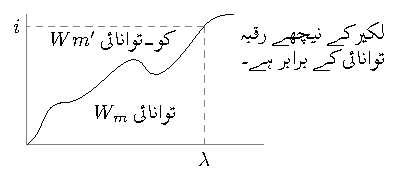
\includegraphics{figEnergyConversionDefiningCoenergy}
\begin{tikzpicture}
%grid
%\draw[gray,thick] (0,0) grid (5,5);
%\draw[gray,thin,xstep=0.1,ystep=0.1] (0,0) grid (5,5);
\pgfmathsetmacro{\l}{5}
 \pgfmathsetmacro{\b}{2.5}
\draw[gray](0,0)--(4,0)node[ right]{};
\draw[gray](0,0)--(0,2.2)node[above]{};
\draw[-] (0,0) to [out=30,in=180] (0.6,0.7) to [out=0,in=120] (2,1.3) to [out=-60,in=-130](3,2) to [out=50,in=180] (3.5,2.2)node[below right,align=left]{\RL{لکیر کے نیچے رقبہ}\\ \RL{ توانائی کے برابر ہے۔}} ;
\draw[dashed,gray](3,0)--(3,2) node[below,black] at (3,0){$\lambda$};
\draw[gray,dashed](3,2)--(0,2) node[left,black]{$i$};
%text
\node[right] at (1,0.5){$W_m$ توانائی};
\node[right] at (0.25,1.75){$W_m' $ \RL{ہم توانائی}};
%
\end{tikzpicture}%
\caption{ہم توانائی کی تعریف۔}
\label{شکل_تبادلہ_توانائی_کو_توانائی_کی_تعریف}
\end{figure}

\begin{align}
W_m'=\lambda i -W_m
\end{align}
ہم توانائی کے جزوی فرق
\begin{align*}
\partial W_m'&=\partial (\lambda i) -\partial W_m\\
&=\lambda \partial i + i \partial \lambda -\partial W_m
\end{align*}
میں مساوات \حوالہ{مساوات_برقی_مقناطیسی_تبادلہ_توانائی_کا_طریقہ}  کا استعمال 
\begin{align*}
\partial W_m'&=\lambda \partial i + i \partial \lambda -(i \partial \lambda-F_m \partial x)
\end{align*}
یعنی
\begin{align}\label{مساوات_تبادلہ_کو_توانائی_تعریفی_مساوات}
\partial W_m'&=\lambda \partial i + F_m \partial x
\end{align}
دیگا۔

یہاں بھی مساوات \حوالہ{مساوات_تبادلہ_جزوی_تفرق_عمومی_الف}  تا  مساوات \حوالہ{مساوات_تبادلہ_توانائی_سے_رو}  کی طرح  کسی بھی تفاعل \عددیء{z(x,y)} کا جزوی فرق 
\begin{align*}
\partial z(x,y)=\frac{\partial z}{\partial x} \dif x+\frac{\partial z}{\partial y} \dif y
\end{align*}
ہو گا لہٰذا ہم توانائی \عددیء{W_m'(x,i)} کا جزوی فرق درج ذیل ہو گا۔
\begin{align}\label{مساوات_تبادلہ_ہمہ_توانائی_جزوی_فرق}
\partial W_m'(x,i)=\frac{\partial W_m'}{\partial x} \dif x+\frac{\partial W_m'}{\partial i} \dif i
\end{align}
مساوات \حوالہ{مساوات_تبادلہ_ہمہ_توانائی_جزوی_فرق} کا مساوات \حوالہ{مساوات_تبادلہ_کو_توانائی_تعریفی_مساوات}  کے ساتھ موازنہ کرنے سے درج ذیل حاصل ہو گا۔
\begin{align}
\lambda&=\left. \frac{\partial W_m'}{\partial i} \right|_{x_0}\label{مساوات_تبادلہ_ارتباط_ہمہ_توانائی}\\
\intertext{اور}
F_m&=\left. \frac{\partial W_m'}{\partial x} \right|_{i_0}\label{مساوات_تبادلہ_کوتوانائی_سے_قوت}
\end{align}
مساوات \حوالہ{مساوات_تبادلہ_کوتوانائی_سے_قوت} قوت دریافت کرنے  کا دوسرا کلیہ دیتی ہے۔ مساوات \حوالہ{مساوات_تبادلہ_کوتوانائی_سے_قوت} میں ہم توانائی  جبکہ مساوات \حوالہ{مساوات_تبادلہ_توانائی_قوت_برقی_رو} میں  توانائی کے ذریعہ قوت  حاصل کی گئی۔

توانائی کے طریقہ  کی طرح مساوات \حوالہ{مساوات_تبادلہ_ارتباط_ہمہ_توانائی} سے درج ذیل تکمل لکھا جا سکتا ہے۔
\begin{align}
W_m'(i_0,x_0)=\int_{0}^{i_0} \lambda(i,x_0) \dif i
\end{align}
جن نظام میں \عددیء{\lambda} اور \عددیء{i} کا تعلق تغیر راست ہو، جس کو مساوات \حوالہ{مساوات_مقناطیسی_دور_خود_امالہ_تعریف} بیان کرتی ہو، ان کے لئے درج بالا تکمل کا حل درج ذیل ہو گا  جہاں \عددیء{i_0}، \عددیء{x_0} کی بجائے عمومی متغیرات \عددیء{i} اور \عددیء{x} لکھے گئے ہیں۔
\begin{align}\label{مساوات_تبادلہ_کوتوانائی_مساوی_امالہ_مربع_رو}
W_m'(i,x)=\int_{0}^{i} L(x) i  \dif i=\frac{L(x) i^2}{2}
\end{align}
بعض مسائل میں توانائی اور  بعض میں ہم توانائی کا استعمال زیادہ آسان ثابت ہوتا ہے۔
%
\ابتدا{مثال}
شکل \حوالہ{شکل_تبادلہ_توانائی_پیچدار_لچھا}  میں ایک پیچدار لچھا دکھایا گیا ہے جس کی محوری لمبائی \عددیء{l}،   رداس \عددیء{r}  اور چکر \عددیء{N}  ہیں۔پیچدار لچھے کے مقناطیسی بہاو کا بیشتر حصہ محوری رخ  لچھے کے اندر رہتا ہے۔ لچھے کے باہر مقناطیسی بہاو کو نظر انداز کرتے ہوئے  لچھے کے اندر محوری لمبائی رخ میدانی شدت \عددیء{H \approx \tfrac{NI}{l}} ہو گی۔
\begin{figure}
\centering
%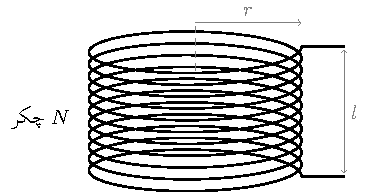
\includegraphics{figEnergyConversionCoil}
\begin{tikzpicture}
%grid
\pgfmathsetmacro{\radX}{1.8}
 \pgfmathsetmacro{\radY}{0.4}
\pgfmathsetmacro{\thetaStart}{0} 
\pgfmathsetmacro{\thetaEnd}{180}
%\draw[gray,thick] (-4*\radX,-4*\radX) grid (4*\radX,4*\radX);
%\draw[gray,thin,xstep=0.1,ystep=0.1] (-4*\radX,-4*\radX) grid (4*\radX,4*\radX);
%coil backside
\foreach \y in {0,0.2,0.4,0.6,0.8,1,1.2,1.4,1.6,1.8,2}{
\draw[thick,domain={0:180},variable=\t,smooth,samples=100] plot({\radX*cos(\t)},{\y+0.1/180*\t+\radY*sin(\t)});
}
%coil front
\foreach \y in {0,0.2,0.4,0.6,0.8,1,1.2,1.4,1.6,1.8,2}{
\draw[thick,domain={180:360},variable=\t,smooth,samples=100] plot({\radX*cos(\t)},{\y+0.1/180*\t+\radY*sin(\t)});
}
%end connections
\draw[thick](\radX,0)--(1.4*\radX,0);
\draw[thick](\radX,2+0.1/180*360)--(1.4*\radX,2+0.1/180*360);
%text
\draw[,<->](1.4*\radX,0+0.05)--(1.4*\radX,2+0.1/180*360-0.05)node[pos=0.5,right]{$l$};
\draw[,dashed](0,2+0.1/180*360-0.4)--(0,2+0.1/180*360+0.4);
\draw[,->] (0,2+0.1/180*360+0.4)--++(\radX,0)node [above,pos=0.5]{$r$};
\draw(-2,1)node[left]{\RL{$N$ چکر}};
\end{tikzpicture}%
\caption{پیچدار لچھا۔}
\label{شکل_تبادلہ_توانائی_پیچدار_لچھا}
\end{figure}

موصل دھات کو امالی برقی توانائی سے پگھلانے کے لئے پیچدار لچھا استعمال کیا جاتا ہے۔میں   \عددیء{100}   تا \عددیء{1500}  کلو واٹ برقی طاقت کی\اصطلاح{امالی برقی بھٹیاں}\فرہنگ{بھٹی}\حاشیہب{high frequency, induction furnaces} بناتا رہا جو بالترتیب  \عددیء{500} تا  \عددیء{1200} ہرٹز پر کام کرتی اور \عددیء{100}  سے  \عددیء{3000} کلوگرام  لوہا پگھلاتی ہیں۔

امالی  بھٹی کے پیچدار لچھے کے اندر غیر موصل پیالے  میں  دھات کے ٹکڑے ڈال کر لچھے میں بدلتا رو گزاری جاتی ہے جو دھات میں بھنور نما امالی برقی رو پیدا کرتی ہے۔  بھنور نما رو دھات کو  گرم کر کے پگھلاتی ہے۔امالی برقی بھٹی میں لوہے کو  \عددیء{1650} ڈگری \اصطلاح{سیلسیئس}\حاشیہب{Celsius, Centigrade} تک گرم کیا جاتا ہے۔

پیچدار لچھے میں برقی رو \عددیء{I_0} کی بنا لچھے پر  رداسی رخ میکانی دباو یعنی قوت فی مربع رقبہ پیدا ہو گا۔میری \عددیء{3000} کلوگرام لوہا پگھلانے کی بھٹی کے پیچدار لچھے کی تفصیل درج ذیل ہے۔
\begin{align*}
N=11, \quad I_0=\SI{10000}{\ampere}, \quad l=\SI{0.94}{\meter}, \quad r=\SI{0.49}{\meter}
\end{align*}
اس پر رداسی رخ میکانی دباو  (نیوٹن فی مربع میٹر)  حاصل کریں۔


حل:\quad 
ہم توانائی کا طریقہ استعمال کرتے ہیں۔
\begin{align*}
L&=\frac{\mu_0 N^2 \pi r^2}{l}\\
W_m'(r,i)&=\frac{L i^2}{2}=\frac{\mu_0 N^2 \pi r^2 I_0^2}{2 l}\\
F&=\frac{\partial W_m'}{\partial r}=\frac{\mu_0 N^2 \pi r I_0^2}{l}
\end{align*}
اس قوت کی علامت  مثبت ہے لہٰذا یہ رداسی رخ  باہر جانب ہو گا۔لچھے کو نلکی تصور کریں جس کی گول سطح  کا رقبہ \عددیء{A=2\pi rl} ہو گا۔یوں میکانی دباو درج ذیل ہو گا۔
\begin{align*}
\frac{F}{A}=\frac{\mu_0 N^2 \pi r I_0^2}{2\pi r l^2}=\frac{\mu_0 N^2  I_0^2}{2 l^2}
\end{align*}
دی گئی معلومات پر کرتے ہوئے درج ذیل  حاصل ہو گا۔
\begin{align*}
\frac{F}{A}=\frac{4\pi 10^{-7} \times 11^2 \times \num{10000}^2 }{2 \times 0.94^2}=\SI{8604}{\newton \per \meter \squared}
\end{align*}
\انتہا{مثال}
%
\ابتدا{مثال}
 \عددیء{2700}  کلوواٹ امالی بھٹی یومیہ \عددیء{70} ٹن\حاشیہد{ہزار کلوگرام ایک ٹن کے برابر ہوتے ہیں۔} لوہا  پگھلاتی\حاشیہد{یہ میں اپنے تجربے کی بنیاد پر کہہ رہا ہوں۔} ہے۔اتنے وزن کی منتقلی کے لئے برقی مقناطیس استعمال کیا جاتا ہے۔شکل \حوالہ{شکل_تبادلہ_توانائی_برقی_مقناطیس} میں ایک ایسا  برقی مقناطیس دکھایا گیا ہے جس کی تفصیل درج ذیل ہے۔
\begin{align*}
N=300, \quad A=\SI{0.8}{\meter \squared}, \quad I=\SI{30}{\ampere}
\end{align*}
برقی مقناطیس اور لوہے کے بیچ اوسط فاصلہ \عددیء{2.5} سنٹی میٹر لیں۔ یہ برقی مقناطیس کتنی کمیت کا لوہا اٹھا سکتا ہے؟
\begin{figure}
\centering
%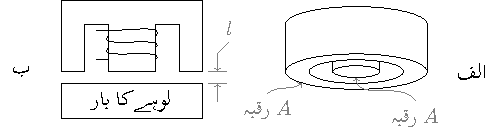
\includegraphics{figEnergyConversionElectroMagnet}
%grid
%\draw[gray,thick] (-4*\radX,-4*\radX) grid (4*\radX,4*\radX);
%\draw[gray,thin,xstep=0.1,ystep=0.1] (-4*\radX,-4*\radX) grid (4*\radX,4*\radX);
\pgfmathsetmacro{\shiftX}{5 cm}
\pgfmathsetmacro{\h}{1.2}
\pgfmathsetmacro{\t}{0.4}
\pgfmathsetmacro{\g}{0.1}
\pgfmathsetmacro{\nL}{3}

\pgfmathsetmacro{\xE}{3*\t cm}
\pgfmathsetmacro{\yE}{\h/4 cm}
\begin{subfigure}{0.45\textwidth}
\centering
\begin{tikzpicture}[x=1cm, y=0.25cm]
\draw(0,0) circle  (1.2);
\draw(0,0) circle  (0.8);
\draw[] (220:1.2) to [out=220,in=45](-1.5,-1.5) node[below] {رقبہ $A$};
\draw[] (-90:0.4) to [out=-90,in=120](1,-2) node[below] {رقبہ $A$};
\begin{scope}
\clip (0,0) circle  (0.8);
\draw(0,0) circle  (0.4);
\draw (-0.4,0)--++(0,2);
\draw (0.4,0)--++(0,2);
\end{scope}
%
\begin{scope}[yshift=0.8cm]
\draw([shift={(0:1.2)}]0,0) arc (0:180:1.2);
\end{scope}
\draw(-1.2,0)--++(0,0.8cm);
\draw(1.2,0)--++(0,0.8cm);
\end{tikzpicture}
\caption{}
\end{subfigure}\hfill
\begin{subfigure}{0.45\textwidth}
\centering
\begin{tikzpicture}
\draw(0,0)--++(0,\h)--++(6*\t,0)--++(0,-\h)--++(-\t,0)--++(0,\h-\t)--++(-\t,0)--++(0,-\h+\t)--++(-2*\t,0)--++(0,\h-\t)--++(-\t,0)--++(0,-\h+\t)--cycle;
\draw(0,-\t/2)--++(6*\t,0)--++(0,-1.5*\t)--++(-6*\t,0)--cycle;     %load
\draw[] (6*\t+0.1,0)--++(0.3,0)coordinate[pos=0.5] (gap);
\draw[] (6*\t+0.1,0)++(0,-\t/2)--++(0.3,0);
\draw[<-] (gap)--++(0,0.3)--++(0.2,0.2) node[above] {$l$};
\draw[<-] (gap)++(0,-0.5*\t)--++(0,-0.3);
\draw node at (3*\t,-1.25*\t){\RL{لوہے کا بوجھ}};
%===================================
\pgfmathsetmacro{\stepHL}{(\h-\t-2*\g)/(\nL)}
%
\def\leftEdge{2*\t};
\def\coilTop{\h-\t-\g};
\def\rightEdge{4*\t};
%
\draw(\leftEdge+\t/4,\coilTop) to [out=0,in=45] (\rightEdge,{\coilTop-\stepHL/2}); %top half turn
%coil itself
\pgfmathsetmacro{\nLend}{\nL-2}
\foreach \y in { 0, ..., \nLend }{
\draw (\leftEdge,{\coilTop-\stepHL/2-\y*\stepHL}) to [out=-135,in=45] (\rightEdge,{\coilTop-\stepHL/2-\y*\stepHL-\stepHL});
} 
%left hand terminals
\draw (\leftEdge+\t/4,\coilTop)--++(-0.75*\t,0) node(TA){};
\draw (\leftEdge,\coilTop-\nL*\stepHL+0.5*\stepHL)--++(-0.5*\t,0)node(TB){};
\end{tikzpicture}
\caption{}
\end{subfigure}
%===========================
%===========================
\caption{برقی مقناطیس۔}
\label{شکل_تبادلہ_توانائی_برقی_مقناطیس}
\end{figure}

حل:
\begin{align*}
L&=\frac{\mu_0 N^2 A}{2 l}\\
W_m'(l,i)&=\frac{L i^2}{2}=\frac{\mu_0 N^2 A i^2}{4 l}\\
F=\frac{\partial W_m'}{\partial l}=-\frac{\mu_0 N^2 A i^2}{4 l^2}&=-\frac{4\pi 10^{-7} \times 300^2 \times 0.8  \times 30^2}{4 \times 0.025^2}
=\SI{-32572}{\newton}
\end{align*}
قوت کی علامت منفی ہے۔یوں یہ مقناطیس اور لوہے کے بیچ فاصلہ کم کرنے کی کوشش کرتی ہے۔ یہ مقناطیس \عددیء{\tfrac{32572}{9.8}=\SI{3324}{\kilo\gram}} کمیت اٹھا سکتا ہے۔
\انتہا{مثال}
%
\ابتدا{مثال}
مثال \حوالہ{مثال_تبادلہ_توانائی_قوت_کا_حصول_بذریعہ_توانائی_طریقہ} کو ہم توانائی کے طریقہ سے حل کریں۔

حل:\quad
مساوات \حوالہ{مساوات_تبادلہ_کوتوانائی_مساوی_امالہ_مربع_رو}   سے
\begin{align*}
W_m'&=\frac{L(x) i^2}{2}=\frac{N^2 \mu_0 w(b-x) i^2}{4 g}
\end{align*}
لکھ کر مساوات \حوالہ{مساوات_تبادلہ_کوتوانائی_سے_قوت}  سے درج ذیل قوت حاصل ہوتی ہے۔
\begin{align*}
F_m=\frac{\partial W'_m}{\partial x}=-\frac{N^2 \mu_0 w i^2}{4 g}=\SI{-28274}{\newton}
\end{align*}
\انتہا{مثال}
%
\حصہ{متعدد لچھوں کا مقناطیسی نظام}
اب تک ایک لچھے کے نظام پر غور کیا گیا۔ اس حصہ میں  ایک سے زیادہ لچھوں کے نظام پر غور کیا جائے گا۔ متعدد لچھوں کا نظام بھی ایک لچھے کے نظام کی طرح حل ہوتے ہیں۔
\begin{figure}
\centering
%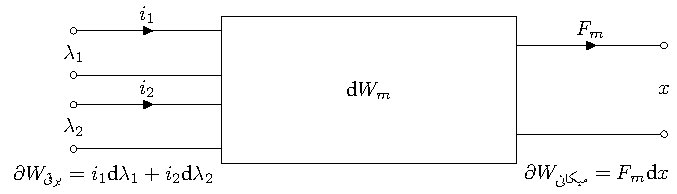
\includegraphics{figEnergyConversionBasicBlockDiagramDetailedTwoCoils}
\begin{tikzpicture}
%grid
%\draw[gray,thick] (0,0) grid (5,5);
%\draw[gray,thin,xstep=0.1,ystep=0.1] (0,0) grid (5,5);
\pgfmathsetmacro{\l}{5}
 \pgfmathsetmacro{\b}{2.5}
\draw (0,0)coordinate(a){}--++(0:\l)coordinate(b){}--++(90:\b)coordinate(c){}--++(180:\l)coordinate(d){}--cycle;
%
\draw($(a)!0.9!(d)$) to [short,-o,i_<={$i_1$}]++(180:\b)coordinate(leftD){};
\draw($(a)!0.6!(d)$) to [short,-o]++(180:\b)coordinate(leftC){};
\draw($(a)!0.4!(d)$) to [short,-o,i_<={$i_2$}]++(180:\b)coordinate(leftB){};
\draw($(a)!0.1!(d)$) to [short,-o]++(180:\b)coordinate(leftA){};
\draw node at ($(leftC)!0.5!(leftD)$){$\lambda_1$};
\draw node at ($(leftA)!0.5!(leftB)$){$\lambda_2$};

\draw($(b)!0.2!(c)$) to [short,-o]++(0:\b)coordinate(rightLow){};
\draw($(b)!0.8!(c)$) to [short,-o,i={$F_m$}]++(0:\b)coordinate(rightUpper){};
\draw node at ($(rightLow)! 0.5 ! (rightUpper)$){$x$};
%
\draw node at (\l/2,\b/2){$\textup{d} W_m$};
\draw[left] node at (0,-0.2){$\partial W_{\textup{برقی}}= i_1 \textup{d}\lambda_1 +i_2 \textup{d}\lambda_2$};
\draw[right] node at (\l,-0.2){$\partial W_{\textup{میکانی}}= F_m \textup{d} x$};
\end{tikzpicture}%
\caption{ دو لچھوں کا نظام۔}
\label{شکل_تبادلہ_توانائی_دو_لچھوں_کا_نظام}
\end{figure}
%
شکل \حوالہ{شکل_تبادلہ_توانائی_دو_لچھوں_کا_نظام}  میں  ایک لچھے کا برقی رو \عددیء{i_1} اور دوسرے لچھے کا برقی رو \عددیء{i_2} ہے۔ اس نظام کے لئے درج ذیل لکھنا ممکن ہے جہاں \عددی{W_m} ذخیرہ توانائی کو ظاہر کرتی ہے۔
\begin{align}
\partial W_{\textup{برقی}}&=i_1 \dif \lambda_1+i_2 \dif \lambda_2\\
\partial W_{\textup{برقی}}&=\partial W_{\textup{میکانی}}+\partial W_m
\end{align}
پہلی مساوات کو دوسری میں پُر کرتے ہوئے درج ذیل مساوات حاصل ہوتی ہے جس میں \عددی{\partial W_{\text{میکانی}}=F_m\dif x} لکھا گیا ہے۔
\begin{align}
i_1 \dif \lambda_1+i_2 \dif \lambda_2&=F_m \dif x+\partial W_m
\end{align}
اس کی ترتیب نو درج ذیل دیگی۔
\begin{align}\label{مساوات_تبادلہ_دو_لچھے_الف}
\partial W_m(\lambda_1,\lambda_2,x)=i_1 \dif \lambda_1+i_2 \dif \lambda_2-F_m \dif x
\end{align}
اب بالکل مساوات \حوالہ{مساوات_تبادلہ_جزوی_تفرق_عمومی_ب}   کی طرح درج ذیل لکھا جا سکتا ہے۔
\begin{align}\label{مساوات_تبادلہ_دو_متغیر_تفرق}
\partial W_m(\lambda_1,\lambda_2,x)=\frac{\partial W_m}{\partial \lambda_1} \dif \lambda_1+\frac{\partial W_m}{\partial \lambda_2} \dif \lambda_2+\frac{\partial W_m}{\partial x} \dif x
\end{align}
مساوات \حوالہ{مساوات_تبادلہ_دو_لچھے_الف} اور \حوالہ{مساوات_تبادلہ_دو_متغیر_تفرق} کے موازنہ سے درج ذیل تعلقات اخذ ہوتے ہیں۔
\begin{align}
i_1&=\left. \frac{\partial W_m(\lambda_1,\lambda_2,x)}{\partial \lambda_1} \right|_{\lambda_2,x}\\
i_2&=\left. \frac{\partial W_m(\lambda_1,\lambda_2,x)}{\partial \lambda_2} \right|_{\lambda_1,x}\\
F_m&=\left. -\frac{\partial W_m(\lambda_1,\lambda_2,x)}{\partial x} \right|_{\lambda_1,\lambda_2}
\end{align}
ان مساوات کا استعمال تب ممکن ہو گا  جب ہمیں توانائی \عددیء{W_m} معلوم ہو لہٰذا ہم پہلے توانائی دریافت کرتے ہیں۔

\begin{figure}
\centering
%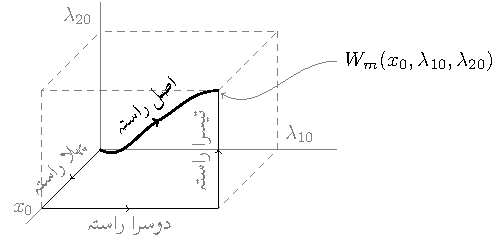
\includegraphics{figEnergyConversionTwoCoilSystemEnergyIntegral}
\begin{tikzpicture}[x={(-0.5cm,-0.5cm)},y={(1cm,0)},z={(0,1cm)}]
%grid
%\draw[gray,thick] (0,0) grid (5,5);
%\draw[gray,thin,xstep=0.1,ystep=0.1] (0,0) grid (5,5);
\pgfmathsetmacro{\x}{2}
\pgfmathsetmacro{\y}{3}
\pgfmathsetmacro{\z}{2} 
%AXIS
\draw[gray](0,0,0)--(2.5,0,0);
\draw[gray](0,0,0)--(0,4,0);
\draw[gray](0,0,0)--(0,0,2.5);
%BOX VECTORS
\draw[->](0,0,0)--++(,0,0) node[gray,above,rotate=45] {\RL{پہلی راہ}};
\draw(\x/2,0,0)--(\x,0,0)node[left,gray]{$x_0$};
\draw[->](\x,0,0)--(\x,\y/2,0)node[gray,below]{\RL{دوسری راہ}};
\draw(\x,\y/2,0)--(\x,\y,0);
\draw[->](\x,\y,0)--(\x,\y,\z/2)node[gray,rotate=90,above]{\RL{تیسری راہ}};
\draw(\x,\y,\z/2)--(\x,\y,\z)coordinate(end);
%dashed
\draw[gray,dashed](end)--++(-\x,0,0)--++(0,-\y,0)node[above left]{$\lambda_{20}$};
\draw[gray,dashed](end)++(-\x,0,0)--++(0,0,-\z)node[above right]{$\lambda_{10}$}--++(\x,0,0);
\draw[gray,dashed](end)--++(0,-\y,0)--++(-\x,0,0);
\draw[gray,dashed](end)++(0,-\y,0)--++(0,0,-\z);
%ACTUAL PATH
\draw[thick,->](0,0,0) to [out=-30,in=-150] (\x/2,\y/2,\y/3)node[black,above,rotate=40]{\RL{اصل راہ}};
\draw[thick] (\x/2,\y/2,\y/3)  to [out=30,in=180] (\x,\y,\z);
%
\draw node[right] at (0,4,1.5){$W_m(x_0, \lambda_{10},\lambda_{20})$};
\draw[gray,<-]  (\x,\y,\z)++(0.1,0.1,0) to [out=-30,in=180](0,4,1.5);
\end{tikzpicture}%
\caption{دو لچھوں کے نظام میں مقناطیسی میدان میں  توانائی۔}
\label{شکل_تبادلہ_توانائی_دو_لچھوں_کے_توانائی_کا_تکمل}
\end{figure}

شکل \حوالہ{شکل_تبادلہ_توانائی_دو_لچھوں_کا_نظام}  میں  لچھوں کو یوں طاقت دی جاتی ہے کہ \عددیء{\lambda_1} اور \عددیء{\lambda_2}  صفر سے  بالترتیب \عددیء{\lambda_{10}}  اور \عددیء{\lambda_{20}}تک  پہنچتے  ہیں اور ساتھ ہی    \عددیء{x} صفر سے تبدیل ہو کر \عددیء{x_0} ہوتا ہے۔ اس عمل کو  شکل \حوالہ{شکل_تبادلہ_توانائی_دو_لچھوں_کے_توانائی_کا_تکمل}  میں موٹی لکیر  سے بطور "اصل راہ" دکھایا گیا  ہے۔ مساوات \حوالہ{مساوات_تبادلہ_توانائی_تکمل_راستہ_دو_ٹکڑے}  کی طرح ذخیرہ توانائی کے تکمل کے لئے درج ذیل  لکھا جا سکتا ہے۔
\begin{align}\label{مساوات_تبادلہ_اصل_راستے_پر_تکمل}
\int\limits_{\text{\RL{اصل راہ}}} \partial W_m=\int\limits_{\text{\RL{پہلی راہ}}} \partial W_m+\int\limits_{\text{\RL{دوسری راہ}}} \partial W_m+\int\limits_{\text{\RL{تیسری راہ}}} \partial W_m
\end{align}
ہم دائیں ہاتھ تکملات کو باری باری حل کرتے ہیں۔

پہلی راہ پر \عددی{\lambda_1} اور \عددی{\lambda_2} صفر رہتے ہیں جبکہ \عددی{x} کی ابتدائی قیمت \عددی{0} اور اختتامی قیمت \عددی{x_0} ہے۔یوں پہلی راہ پر تکمل درج ذیل ہو گا۔
\begin{align}\label{مساوات_تبادلہ_پہلی_راہ_دو_لچھے_الف}
\int\limits_{\text{\RL{پہلی راہ}}} \partial W_m=\int_{0}^{0} i_1 \dif \lambda_1+\int_{0}^{0} i_2 \dif \lambda_2-\int_0^{x_0} F_m \dif x
\end{align}
کسی بھی تکمل کا ابتدائی  اور اختتامی  نقطہ ایک دوسرے جیسا ہونے کی صورت میں  تکمل کی قیمت صفر ہوتی ہے لہٰذا درج بالا میں دائیں ہاتھ، پہلے دو تکملات صفر ہوں گے:
\begin{align}\label{مساوات_تبادلہ_پہلی_راہ_دو_لچھے_ب}
\int_{0}^{0} i_1 \dif \lambda_1=\int_{0}^{0} i_2 \dif \lambda_2=0
\end{align}
پہلی راہ پر \عددیء{\lambda_1} اور \عددیء{\lambda_2} صفر ہیں،یعنی، دونوں لچھوں میں برقی رو صفر ہے، لہٰذا مقناطیسی بہاو اور قوت \عددیء{F_m} صفر ہوں گے۔ یوں   مساوات \حوالہ{مساوات_تبادلہ_پہلی_راہ_دو_لچھے_الف} میں قوت کا تکمل صفر ہو گا۔
\begin{align}\label{مساوات_تبادلہ_پہلی_راہ_دو_لچھے_پ}
\int_0^{x_0} F_m \dif x&=\int_0^{x_0} 0 \dif x=0&&\text{\RL{\small{(صفر کا تکمل صفر ہو گا)}}}
\end{align}
مساوات \حوالہ{مساوات_تبادلہ_پہلی_راہ_دو_لچھے_ب} اور مساوات \حوالہ{مساوات_تبادلہ_پہلی_راہ_دو_لچھے_پ} کے نتائج کے تحت پہلی راہ پر تکمل صفر ہو گا۔
\begin{align}\label{مساوات_تبادلہ_پہلا_راستہ_جزو}
\int\limits_{\text{\RL{پہلی راہ}}} \partial W_m=0
\end{align}

دوسری راہ پر  \عددی{\lambda_1} کی ابتدائی قیمت \عددی{0} اور اختتامی قیمت \عددی{\lambda_{10}} ہے، \عددی{\lambda_2} صفر رہتا ہے  جبکہ \عددی{x} کی قیمت \عددی{x_0} رہتی ہے۔ یوں دوسری راہ پر تکمل درج ذیل ہو گا۔
\begin{align}\label{مساوات_تبادلہ_دوسری_راہ_الف}
\int\limits_{\text{\RL{دوسری راہ}}} \partial W_m=\int_{0}^{\lambda_{10}} i_1 \dif \lambda_1+\int_{0}^{0} i_2 \dif \lambda_2-\int_{x_0}^{x_0} F_m \dif x
\end{align}
تکمل کا ابتدائی اور اختتامی  نقطہ ایک جیسا ہونے کی صورت میں  تکمل   صفر ہو گا:
\begin{align*}
\int_{0}^{0} i_2 \dif \lambda_2=\int_{x_0}^{x_0} F_m \dif x=0
\end{align*}
یوں مساوات \حوالہ{مساوات_تبادلہ_دوسری_راہ_الف} درج ذیل صورت اختیار کرتی ہے۔
\begin{align}\label{مساوات_تبادلہ_دوسرا_راستہ_توانائی}
\int\limits_{\text{\RL{دوسری راہ}}} \partial W_m=\int_{0}^{\lambda_{10}} i_1 \dif \lambda_1
\end{align}
یہاں مساوات \حوالہ{مساوات_مقناطیسی_دور_ارتباط_دو_لچھے} ، \حوالہ{مساوات_مقناطیسی_دور_دوسرے_لچھے_کی_ارتباط}  اور \حوالہ{مساوات_مقناطیسی_دور_مشترکہ_امالہ_یکساں}   کی ضرورت پیش آئے گی جنہیں دوبارہ پیش کرتے ہیں۔
\begin{align}
\lambda_1&=L_{11} i_1+L_{12} i_2\label{مساوات_تبادلہ_دوبارہ_پیش_الف}\\
\lambda_2&=L_{21} i_1+L_{22} i_2\label{مساوات_تبادلہ_دوبارہ_پیش_ب}\\
L_{12}&=L_{21}  \label{مساوات_تبادلہ_دوبارہ_پیش_پ}
\end{align}
مساوات \حوالہ{مساوات_تبادلہ_دوبارہ_پیش_الف} اور مساوات \حوالہ{مساوات_تبادلہ_دوبارہ_پیش_ب} کو \عددیء{i_1}  اور \عددیء{i_2} کے لئے حل کے
\begin{align}
i_1&=\frac{L_{22} \lambda_1-L_{12} \lambda_2}{D} \label{مساوات_تبادلہ_رو_نمبر_ایک}\\
i_2&=\frac{L_{11} \lambda_2-L_{21} \lambda_1}{D} \label{مساوات_تبادلہ_رو_نمبر_دو}
\end{align}
حاصل ہو گا جہاں \عددی{D} درج ذیل ہے۔
\begin{align*}
D=L_{11}L_{22}-L_{12}L_{21}
\end{align*}
مساوات  \حوالہ{مساوات_تبادلہ_دوسرا_راستہ_توانائی} کو مساوات \حوالہ{مساوات_تبادلہ_رو_نمبر_ایک}  کے برابر ٹھرا کر،  دوسری راہ پر  \عددیء{\lambda_2} صفر لے کر  درج ذیل حاصل ہو گا۔
\begin{align*}
\int_0^{\lambda_{10}} \left( \frac{L_{22} \lambda_1-L_{12} \lambda_2}{D}\right) \dif \lambda_1=\frac{L_{22}}{D}\int_0^{\lambda_{10}} \lambda_1 \dif \lambda_1=\frac{L_{22}\lambda_{10}^2}{2D}
\end{align*}
یوں دوسری راہ پر تکمل کی قیمت درج ذیل ہو گی۔
\begin{align}\label{مساوات_تبادلہ_دوسرہ_راستہ_جزو}
\int\limits_{\text{\RL{دوسری راہ}}} \partial W_m=\frac{L_{22}\lambda_{10}^2}{2D}
\end{align}
تیسری راہ پر \عددی{\lambda_1} کی قیمت \عددی{\lambda_{10}} اور \عددی{x} کی قیمت \عددی{x_0} پر برقرار رہتی ہے جبکہ \عددی{\lambda_2} کی ابتدائی قیمت \عددی{0} اور اختتامی قیمت \عددی{\lambda_{20}} ہے۔  یوں تیسری راہ پر تکمل درج ذیل ہو گا۔
\begin{align}\label{مساوات_تبادلہ_تیسری_راہ_الف}
\int\limits_{\text{\RL{تیسری راہ}}} \partial W_m=\int_{\lambda_{10}}^{\lambda_{10}} i_1 \dif \lambda_1+\int_{0}^{\lambda_{20}} i_2 \dif \lambda^2_2-\int_{x_0}^{x_0} F_m \dif x
\end{align}
تکمل کا ابتدائی اور اختتامی  نقطہ ایک جیسا ہونے کی صورت میں تکمل کی قیمت صفر ہوتی ہے لہٰذا درج بالا میں دائیں ہاتھ پہلا اور تیسرا تکمل صفر ہو گا:
\begin{align}\label{مساوات_تبادلہ_تیسری_راہ_نتائج_الف}
\int_{\lambda_{10}}^{\lambda_{10}} i_1 \dif \lambda_1=\int_{x_0}^{x_0} F_m \dif x=0
\end{align}
مساوات \حوالہ{مساوات_تبادلہ_رو_نمبر_دو} کی استعمال سے  مساوات \حوالہ{مساوات_تبادلہ_تیسری_راہ_الف} کا باقی حصہ حل کرتے ہیں۔ 
\begin{gather}
\begin{aligned}\label{مساوات_تبادلہ_تیسری_راہ_نتائج_ب}
\int_{0}^{\lambda_{20}} i_2 \dif \lambda_2&=\int_{0}^{\lambda_{20}} \left(\frac{L_{11} \lambda_2-L_{21} \lambda_{10}}{D} \right) \dif \lambda_2\\
&=\frac{L_{11}}{D}\int_{0}^{\lambda_{20}} \lambda_2 \dif \lambda_2-\frac{L_{21}\lambda_{10}}{D}\int_0^{\lambda_{20}} \dif \lambda_2\\
&=\frac{L_{11} \lambda^2_{20}}{2D}-\frac{L_{21}\lambda_{10} \lambda_{20}}{D}
\end{aligned}
\end{gather}
مساوات \حوالہ{مساوات_تبادلہ_تیسری_راہ_نتائج_الف} اور مساوات \حوالہ{مساوات_تبادلہ_تیسری_راہ_نتائج_ب} کی نتائج سے  تیسری راہ کا تکمل درج ذیل حاصل ہو گا۔
\begin{align}\label{مساوات_تبادلہ_تیسرہ_راستہ_جزو}
\int\limits_{\text{\RL{تیسری راہ}}} \partial W_m=\frac{L_{11} \lambda_{20}^2}{2D}-\frac{L_{21}\lambda_{10} \lambda_{20}}{D}
\end{align}

مساوات \حوالہ{مساوات_تبادلہ_پہلا_راستہ_جزو} ،\حوالہ{مساوات_تبادلہ_دوسرہ_راستہ_جزو}  اور \حوالہ{مساوات_تبادلہ_تیسرہ_راستہ_جزو}   کو جمع کر کے مساوات \حوالہ{مساوات_تبادلہ_اصل_راستے_پر_تکمل}   کا درج ذیل حل حاصل ہو گا جہاں \عددیء{\lambda_{10}}، \عددیء{\lambda_{20}}، \عددیء{x_0} کی جگہ عمومی متغیرات \عددیء{\lambda_1}، \عددیء{\lambda_2}، \عددیء{x} لکھے گئے ہیں۔
\begin{align}\label{مساوات_تبادلہ_اصل_راستے_تکمل_کا_جواب}
W_m(x,\lambda_1,\lambda_2)=\frac{L_{22} \lambda_{1}^2}{2D}+\frac{L_{11} \lambda_{2}^2}{2D}-\frac{L_{21}\lambda_{1} \lambda_{2}}{D}
\end{align}


دو لچھوں کے نظام میں  ہم توانائی کی تعریف
\begin{align*}
W_m'=i_1\lambda_1+i_2\lambda_2-W_m
\end{align*}
ہو گی۔ یوں درج ذیل ہو گا۔
\begin{align*}
\partial W_m'=i_1\partial \lambda_1+\lambda_1\partial i_1+i_2\partial \lambda_2+\lambda_2\partial i_2-\partial W_m
\end{align*}
مساوات \حوالہ{مساوات_تبادلہ_دو_لچھے_الف} استعمال کرتے ہوئے ہم توانائی کے جزوی فرق کی مساوات حاصل ہو گی:
\begin{align}
\partial W_m'(x,i_1,i_2)=\lambda_1 \dif i_1+\lambda_2 \dif i_2+F_m \dif x
\end{align}
جبکہ \عددی{\lambda_1}، \عددی{\lambda_2} اور \عددی{F_m} کی مساواتیں درج ذیل ہوں گی۔
\begin{align}
\lambda_1&=\left. \frac{\partial W_m'(x,i_1,i_2)}{\partial i_1} \right|_{x,i_2}\\
\lambda_2&=\left. \frac{\partial W_m'(x,i_1,i_2)}{\partial i_2} \right|_{x,i_1}\\
F_m&=\left. \frac{\partial W_m'(x,i_1,i_2)}{\partial x} \right|_{i_1,i_2}
\end{align}
مساوات \حوالہ{مساوات_تبادلہ_اصل_راستے_تکمل_کا_جواب}  کی مقابل ہم توانائی کی مساوات درج ذیل ہو گی۔
\begin{align}
W_m'(x,i_1,i_2)=\frac{1}{2}L_{11}(x) i_1^2+\frac{1}{2} L_{22}(x) i_2^2+L_{12}(x)i_1 i_2
\end{align}
ہم قوت کو ہم توانائی سے  حاصل کرتے ہیں:
\begin{align}
F_m=\left. \frac{\partial W_m'(x,i_1,i_2)}{\partial x} \right|_{i_1,i_2}=\frac{i_1^2}{2} \frac{\dif L_{11}(x)}{\dif x}+\frac{i_2^2}{2}\frac{\dif L_{22}(x)}{\dif x}+i_1 i_2 \frac{\dif L_{12}(x)}{\dif x}
\end{align}
%
\ابتدا{مثال}
شکل \حوالہ{شکل_تبادلہ_توانائی_دو_لچھوں_کا_نظام}  میں میکانی کام کو \عددیء{\partial W_{\textup{میکانی}}=T_m \dif \theta}  لکھ کر توانائی کے طریقہ سے حل کریں۔

حل: \quad 
توانائی کی مساوات
\begin{align*}
\partial W_{\textup{برقی}}&=\partial W_{\textup{میکانی}}+\partial W_m
\end{align*}
میں
\begin{align*}
\partial W_{\textup{برقی}}&=i_1 \dif \lambda_1+i_2 \dif \lambda_2
\end{align*}
اور  \عددیء{\partial W_{\textup{میکانی}}=T_m \dif \theta} پر کر کے ترتیب نو سے  درج ذیل حاصل ہو گا۔
\begin{align}\label{مساوات_تبادلہ_مروڑ_الف}
\partial W_m=i_1 \dif \lambda_1+i_2 \dif \lambda_2-T_m\dif \theta
\end{align}
\عددیء{W_m} کے جزوی فرق
\begin{align*}
\partial W_m(\lambda_1,\lambda_2,\theta)=\frac{\partial W_m}{\partial \lambda_1}\dif \lambda_1+\frac{\partial W_m}{\partial \lambda_2}\dif \lambda_2+\frac{\partial W_m}{\partial \theta}\dif \theta
\end{align*}
کا مساوات \حوالہ{مساوات_تبادلہ_مروڑ_الف} کے ساتھ موازنہ کرنے سے درج ذیل اخذ کیے جا سکتے ہیں۔
\begin{align}
i_1&=\left. \frac{\partial W_m(\lambda_1,\lambda_2,\theta)}{\partial \lambda_1} \right|_{\lambda_2,\theta}\\
i_2&=\left. \frac{\partial W_m(\lambda_1,\lambda_2,\theta)}{\partial \lambda_2} \right|_{\lambda_1,\theta}\\
T_m&=-\left. \frac{\partial W_m(\lambda_1,\lambda_2,\theta)}{\partial \theta} \right|_{\lambda_1,\lambda_2}\label{مساوات_تبادلہ_مروڑ_توانائی_حل}
\end{align}
مساوات \حوالہ{مساوات_تبادلہ_مروڑ_الف}  عین مساوات \حوالہ{مساوات_تبادلہ_دو_لچھے_الف}  کی مانند ہے۔مساوات \حوالہ{مساوات_تبادلہ_مروڑ_الف}  حل کرنے کا ایک ایک قدم  مساوات \حوالہ{مساوات_تبادلہ_دو_لچھے_الف}  حل کرنے کی طرح ہے، بس فاصلہ \عددیء{x} کی جگہ زاویہ \عددیء{\theta} آئے گا۔یوں جواب میں میدانی توانائی کے متغیرات  \عددیء{\lambda_1,\lambda_2,\theta} ہوں گے:
\begin{align}\label{مساوات_گھومتے_مشین_توانائی_بذریعہ_تکمل}
W_m(\lambda_{1},\lambda_{2},\theta)=\frac{L_{22} \lambda_{1}^2}{2D}+\frac{L_{11} \lambda_{2}^2}{2D}-\frac{L_{21} \lambda_{1} \lambda_{2}}{D}
\end{align}

اسی طرح ہم توانائی کے لئے درج ذیل ہو گا۔
\begin{align}
\partial W_m'(i_1,i_2,\theta)=\lambda_1 \dif i_1+\lambda_2 \dif i_2+T_m \dif \theta
\end{align}
%
\begin{gather}
\begin{aligned}\label{مساوات_تبادلہ_کوتوانائی_سے_مروڑ}
\lambda_1&=\left.\frac{\partial W_m'(i_1,i_2,\theta)}{\partial i_1} \right|_{i_2,\theta}\\
\lambda_2&=\left.\frac{\partial W_m'(i_1,i_2,\theta)}{\partial i_2} \right|_{i_1,\theta}\\
T_m&=\left.\frac{\partial W_m'(i_1,i_2,\theta)}{\partial \theta} \right|_{i_1,i_2}
\end{aligned}
\end{gather}
ہم توانائی کی مساوات درج ذیل ہو گی۔
\begin{align}\label{مساوات_تبادلہ_کوتوانائی_از_خود}
W_m'(i_1,i_2,\theta)=\frac{1}{2} L_{11} i_1^2+\frac{1}{2} L_{22} i_2^2+L_{12} i_1 i_2
\end{align}
\انتہا{مثال}
%
\ابتدا{مثال}
شکل \حوالہ{شکل_تبادلہ_توانائی_دو_لچھوں_میں_مروڑ}  میں دو لچھوں کا نظام دکھایا گیا ہے۔اس نظام کا ایک حصہ ساکن رہتا ہے اور دوسرا گھوم سکتا ہے۔افقی لکیر سے گھڑی کی سوئیوں  کے مخالف رخ گھومتے ہوئے  زاویہ \عددیء{\theta}  ناپا جاتا ہے۔لچھوں کی خود امالہ اور مشترکہ امالہ مندرجہ ذیل ہیں۔
\begin{align*}
L_{11}&=20+30\cos 2 \theta\\
L_{22}&=\left(20+30\cos 2\theta \right) \times 10^{-3}\\
L_{12}&=0.15 \cos \theta
\end{align*}
 برقی رو  \عددیء{i_1=\SI{0.02}{\ampere},i_2=\SI{5}{\ampere}} پر قوت مروڑ \عددیء{T_m} معلوم کریں۔
\begin{figure}
\centering
%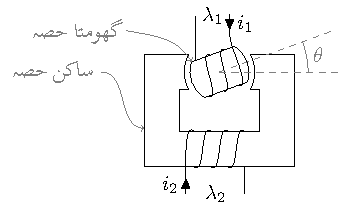
\includegraphics{figEnergyConversionShowingRotor}
\begin{tikzpicture}
%grid
%\draw[gray,thick] (0,0) grid (5,5);
%\draw[gray,thin,xstep=0.1,ystep=0.1] (0,0) grid (5,5);
\pgfmathsetmacro{\r}{0.5}
\pgfmathsetmacro{\g}{0.1}
\pgfmathsetmacro{\angle}{30} 
\pgfmathsetmacro{\angleRotation}{20} 
\pgfmathsetmacro{\angleR}{40}
\pgfmathsetmacro{\t}{2*(\r+\g)*sin(\angle)}
\pgfmathsetmacro{\tr}{2*\r*sin(\angleR)}
\pgfmathsetmacro{\hor}{(\r+\g)*cos(\angle)}
\pgfmathsetmacro{\leg}{0.75}
\pgfmathsetmacro{\w}{2*(\hor+\leg)}
\pgfmathsetmacro{\h}{0.75*\w}
%STATOR
\draw([shift={(-\angle:\r+\g)}]0,0) arc (-\angle:\angle:\r+\g)--++(\leg,0)--++(0,-\h)--++(-\w,0)--++(0,\h)--++(\leg,0)  arc (180-\angle:180+\angle:\r+\g)--++(-\leg+\t,0)--++(0,-\h+2*\t)--++(\w-2*\t,0)--++(0,\h-2*\t)--++(-\leg+\t,0);
\draw[]  (-\r-2*\leg,0) node[left] {\RL{ساکن حصہ}}  to [out=0,in=180] (-\w/2,-\h/2);
%
%============
\begin{scope}[rotate=90]
%COIL ON STATOR
\pgfmathsetmacro{\nL}{4}
\pgfmathsetmacro{\stepHL}{(\w-2*\t-2*\g)/(\nL)}
%
\def\leftEdge{-\h+\t/2};
\def\coilTop{\w/2-\g-\t};
\def\rightEdge{-\h+1.5*\t};
%
\draw(\leftEdge+\t/4,\coilTop) to [out=0,in=45] (\rightEdge,{\coilTop-\stepHL/2}); %top half turn
%coil itself
\pgfmathsetmacro{\nLend}{\nL-2}
\foreach \y in { 0, ..., \nLend }{
\draw (\leftEdge,{\coilTop-\stepHL/2-\y*\stepHL}) to [out=-135,in=45] (\rightEdge,{\coilTop-\stepHL/2-\y*\stepHL-\stepHL});
} 
%left hand terminals
\draw (\leftEdge+\t/4,\coilTop)--++(-0.5*\t,0) coordinate(TRA){};
\draw (\leftEdge,\coilTop-\nL*\stepHL+0.5*\stepHL)--++(-0.25*\t,0)coordinate(TRB){};
\end{scope}
\draw(TRA) to [short,i_<={$i_2$}] ++(0,-0.3)node (TRAA){};
\draw(TRB) to [short] ++(0,-0.3)node(TRBB){};
\node at ($(TRAA)!0.5!(TRBB)$){$\lambda_2$};
%========
%ROTOR
\begin{scope}[rotate=\angleRotation]
\pgfmathsetmacro{\hRot}{\r*cos(\angleR)}
\draw([shift={(-\angleR:\r)}]0,0) arc (-\angleR:\angleR:\r)--++(-2*\hRot,0) arc (180-\angleR:180+\angleR:\r)--++(2*\hRot,0);
%
\draw[]  (-\r-1*\leg,1.2) node[left] {\RL{گھومتا حصہ}}  to [out=-30,in=100] (180-\angleR:\r);
\end{scope}
%=================
%ROTOR COIL
\begin{scope}[rotate=-90+\angleRotation]
\pgfmathsetmacro{\nL}{3}
\pgfmathsetmacro{\stepHL}{(2*\r-2*\g)/(\nL)}
%
\def\leftEdge{-\tr/2};
\def\coilTop{\r-1.5*\g};
\def\rightEdge{\tr/2};
%
\draw(\leftEdge+\tr/4,\coilTop) to [out=0,in=45] (\rightEdge,{\coilTop-\stepHL/2}); %top half turn
%coil itself
\pgfmathsetmacro{\nLend}{\nL-2}
\foreach \y in { 0, ..., \nLend }{
\draw (\leftEdge,{\coilTop-\stepHL/2-\y*\stepHL}) to [out=-135,in=45] (\rightEdge,{\coilTop-\stepHL/2-\y*\stepHL-\stepHL});
} 
%left hand terminals
\draw (\leftEdge+\tr/4,\coilTop)coordinate(kA);%--++(-0.5*\tr,0) coordinate(TA){};
\draw (\leftEdge,\coilTop-\nL*\stepHL+0.5*\stepHL)coordinate(kB);% to [out=180,in=90]++(-0.25*\t,0)coordinate(TB){};
%==================
\end{scope}
%
\draw(kA) to [out=110,in=-90]++(-0.1,0.4) to [short,i_<={$i_1$}] ++(0,0.3)node(rTA){};
\draw(kB) to [out=100,in=-90]++(0,0.2) to [short] ++(0,0.55)node(rTB){};
\draw node at ($(rTA)!0.5!(rTB)$){$\lambda_1$};
%
\draw[dashed](0,0) --++(0:2);
\draw[dashed](0,0) --++(\angleRotation:2);
\draw[-stealth]([shift={(0:1.5)}]0,0) arc (0:\angleRotation:1.5);
\draw[] node at (\angleRotation/2:1.7){$\theta$};
\end{tikzpicture}
\caption{دو لچھوں کے نظام میں قوت مروڑ۔}
\label{شکل_تبادلہ_توانائی_دو_لچھوں_میں_مروڑ}
\end{figure}

حل:\quad
مساوات \حوالہ{مساوات_تبادلہ_کوتوانائی_از_خود} ہم توانائی دیتی ہے۔
\begin{align*}
W_m'=\frac{1}{2}(20+30\cos 2\theta)i_1^2+\frac{1}{2}(20+30\cos 2\theta)(10^{-3})i_2^2+(0.15\cos\theta)i_1i_2
\end{align*}
مساوات \حوالہ{مساوات_تبادلہ_کوتوانائی_سے_مروڑ}  کا آخری جزو قوت مروڑ دیتی ہے۔
\begin{align*}
T_m=\frac{\partial W_m'}{\partial \theta}&=-30 i_1^2 \sin 2 \theta-30\times 10^{-3} i_2^2 \sin 2 \theta -0.15 i_1 i_2 \sin \theta\\
&=-0.012 \sin 2 \theta-0.75 \sin 2 \theta-0.015 \sin \theta\\
&=-0.762 \sin 2 \theta-0.015 \sin \theta
\end{align*}
قوت مروڑ کی علامت منفی ہے لہٰذا یہ زاویہ میں تبدیلی کی مخالفت کرے گا۔یوں اگر آپ زاویہ بڑھائیں (مثبت \عددی{\theta}) تو یہ نظام زاویہ کم کرنے کے رخ قوت مروڑ (منفی \عددی{T_m}) پیدا کرے گا اور اگر آپ زاویہ کم (منفی \عددی{\theta}) کرنے کی کوشش کریں تو یہ نظام  زاویہ بڑھانے کے رخ قوت مروڑ (مثبت \عددی{T_m}) پیدا کرے گا۔سادہ زبان میں گھومتا حصہ اُفقی لکیر پر رہنے کی کوشش کرے گا۔
\انتہا{مثال}
